 \documentclass[11.5pt]{article}
\usepackage[table]{xcolor}
\definecolor{lightgray}{gray}{0.9}
\usepackage{multirow} 
\usepackage{lscape}
\usepackage{filecontents}
\usepackage[left=2.5cm,top=2.5cm,right=2.5cm,bottom=2.5cm]{geometry}
\usepackage{amsmath}
\usepackage{array}
\usepackage{caption}
\usepackage{longtable}
\usepackage{placeins}
\usepackage{graphicx}
\usepackage{subcaption}
\usepackage{setspace}
%\usepackage[active,tightpage]{preview}
\usepackage{natbib}
\bibpunct{(}{)}{,}{a}{}{;} 
\usepackage{url}
\usepackage{nth}	
\usepackage{authblk}
\usepackage{listings}
% for the d in integrals
\newcommand{\dd}{\; \mathrm{d}}
\newcommand{\tc}{\quad\quad\text{,}}
\newcommand{\tp}{\quad\quad\text{.}}
\bibliographystyle{apalike}

\title{Additional file 1 for the article: Stagnation, deterioration and disparities on adulthood survival in Mexican states, 1990-2015.}

\author[1]{Jos\'e Manuel Aburto}
\author[2]{Tim Riffe}
\author[1]{Vladimir Canudas-Romo}
\affil[1]{Department of Public Health \& Max Planck Odense Center on the Biodemography of Aging at University of Southern Denmark}
\affil[2]{Max Planck Institute for Demographic Research}


\begin{document}

\maketitle

\newpage

\section*{Supplemental material}
Appendix Table 1. Definitions of cause-of-death categories using the \nth{9} and \nth{10} revision of the International Classification of Diseases.\\

{\renewcommand{\baselinestretch}{1}\selectfont

\begin{longtable}{p{8cm}p{4cm}p{4cm}ccc}
\hline
\textbf{Category} & \textbf{ICD-10} & \textbf{ICD-9}\\
\hline
\endfirsthead
\multicolumn{3}{c}%
{\tablename\ \thetable\ -- \textit{Continue}} \\
\hline
\textbf{Category} & \textbf{ICD-10} & \textbf{ICD-9}\\
\hline
\endhead
\hline \multicolumn{3}{r}{\textit{Continues}} \\
\endfoot
\hline
\endlastfoot
\multicolumn{3}{l}{\bf I. Amenable to medical service}  \\
 I.A. AM-Infectious \& respiratory diseases : intestinal infections, tuberculosis, zoonotic bacterial diseases, other bacterial diseases, septicemia, poliomyelitis, measles, rubella, infectious hepatitis, ornithosis, rickettsioses/ arthropod-borne, syphilis (all forms), yaws, respiratory diseases, influenza \& pneumonia, chronic lower respiratory diseases & A00-A09, A16-A19, B90, A20-A26, A28, A32, A33, A35, A36, A37, A40-A41, A80, B05-B06, B15-B19, A70, A68, A75, A77, A50-A64, A66, J00-J08, J20-J39, J60-J99, J09-J18, J40-J47 & 001-009, 010-018, 32, 33, 37, 137, 020-027, 38, 45, 55-56, 70, 73, 080-082, 087, 090-099, 102, 460-479, 500-519, 480-488, 490-496 \\
           I.B. AM-Cancers: malignant neoplasm of colon, skin, breast, cervix, prostate, testis, bladder, kidney-Wilm's tumor only, eye, thyroid carcinoma, Hodgkin’s disease, leukemia & C16,C18-C21, C43-C44, C50, C53, C61, C62, C67, C64, C69, C73, C81, C91-C95 & 153-154, 172-173, 174, 180, 185, 186, 188-189, 190, 193, 201, 204-208\\
           I.C. AM-Circulatory: active/acute rheumatic fever, chronic rheumatic heart disease, hypertensive disease, cerebrovascular disease & I00-I02, I05-I09, I10-I13, I15, I60-I69 & 390-392, 393-398, 401-405, 430-438\\
          I.D. AM-Birth: maternal deaths (all), congenital cardiovascular anomalies, perinatal deaths (excluding stillbirths) & O00-O99, Q20-Q28, P00-P96 & 630-676, 745-747, 760-779\\
          I.E. AM-Other: disease of thyroid, epilepsy, peptic ulcer, appendicitis, abdominal hernia, cholelithiasis \& cholecystitis, nephritis, benign prostatic hyperplasia, misadventures to patients during surgical or medical care, cisticerchosis & E00-E07, 40-G41, K25-K27, K35-K38, K40-K46, K80-K81,  N00-N07, N17-N19, N25-N27, N40, Y60-Y69, Y83-Y84, B69 & 240-246, 345, 531-533, 540-543, 550-553, 574-575.1, 580-589, 600, E870-E876, E878-E879\\
 & \\          
 {\bf II. Diabetes}  & E10-E14 & 250 \\      
 & \\
 {\bf III. Ischemic Heart Diseases (IHD)}   & I20-I25 & 410-414, 429.2\\
 & \\           
 {\bf IV. HIV/AIDS} & B20-B24 & 279.1, 042-044\\ 
  & \\                
{\bf V. Lung cancer}  & C33-C34 & 162\\
  & \\          
{\bf VI. Cirrhosis}&  K70 & 571.1-571.3\\
 & \\          
{\bf VII. Homicides}  & X85-Y09 & E960-E969\\     
 & \\           
 {\bf VIII. Road traffic accidents}  & V01-V99 & E810-E819 \\     
 & \\           
{\bf IX. Suicide and self-inflicted injuries}  & U03, X60-X84, Y87.0 & E950-E959\\ 
 & \\          
{\bf X. Residual Causes }:  other cancers and other heart diseases & C00-D48, I00-I99 if not listed above, R00-R99 & 140-239, 390-459 if not listed above, 780-799
\label{ME_Mex}
\end{longtable}



\subsection*{Temporary Life Expectancy}
Temporary life expectancy between ages
$x_1$ and $x_2$, for $x_1<x_2$, is defined as the average years of life lived between these ages according to a given set of mortality rates \citep{arriaga1984}. We denote this quantity as
$_{(x_2-x_1)}e_{x_1}$, and its benchmark minimum as $_{(x_2-x_1)}e^{\star}_{x_1}$. Defined in
terms of lifetable survivorship, $\ell(x)$:

\begin{equation}
_{(x_2-x_1)}e_{x_1} = \frac{\int _{x_1}^{x_2} \ell(x) \dd x}{\ell(x_1)}
\end{equation}

If full survival is achieved, the maximum life expectancy is $x_2-x_1$.  For example, if we set $x_1=0$ and $x_2=14$, if no person dies between the ages 0 and 14, on average the population lives 14 full years.



\begin{figure}
\centering
\caption{Cause-specific mortality counts, 1990-2010.}
\label{fig:ClassSens}
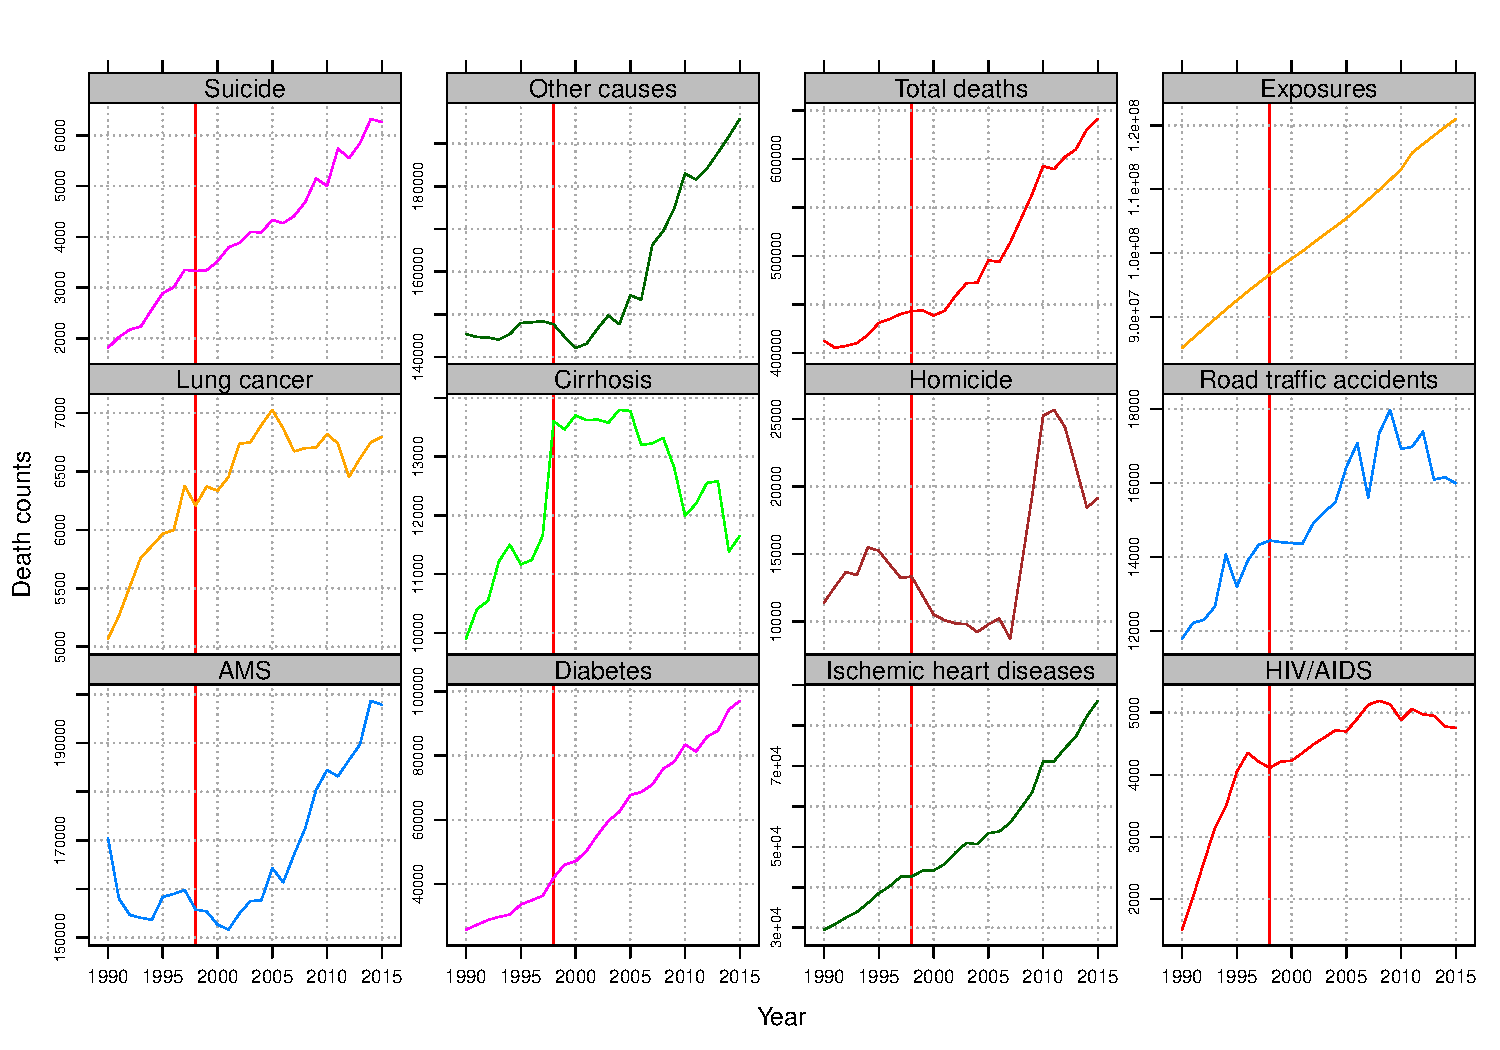
\includegraphics[scale=.6]{Sensitivity_fig.pdf}

Note: AMS ``amenable to medical service''. The red line indicates the change from ICD 9 to ICD 10. 
\end{figure}

\begin{figure}[h!]
\centering
\caption{Inequality in life expectancy by age group measured by the Gini coefficient, 1990-2015.}
\label{fig:Gini}
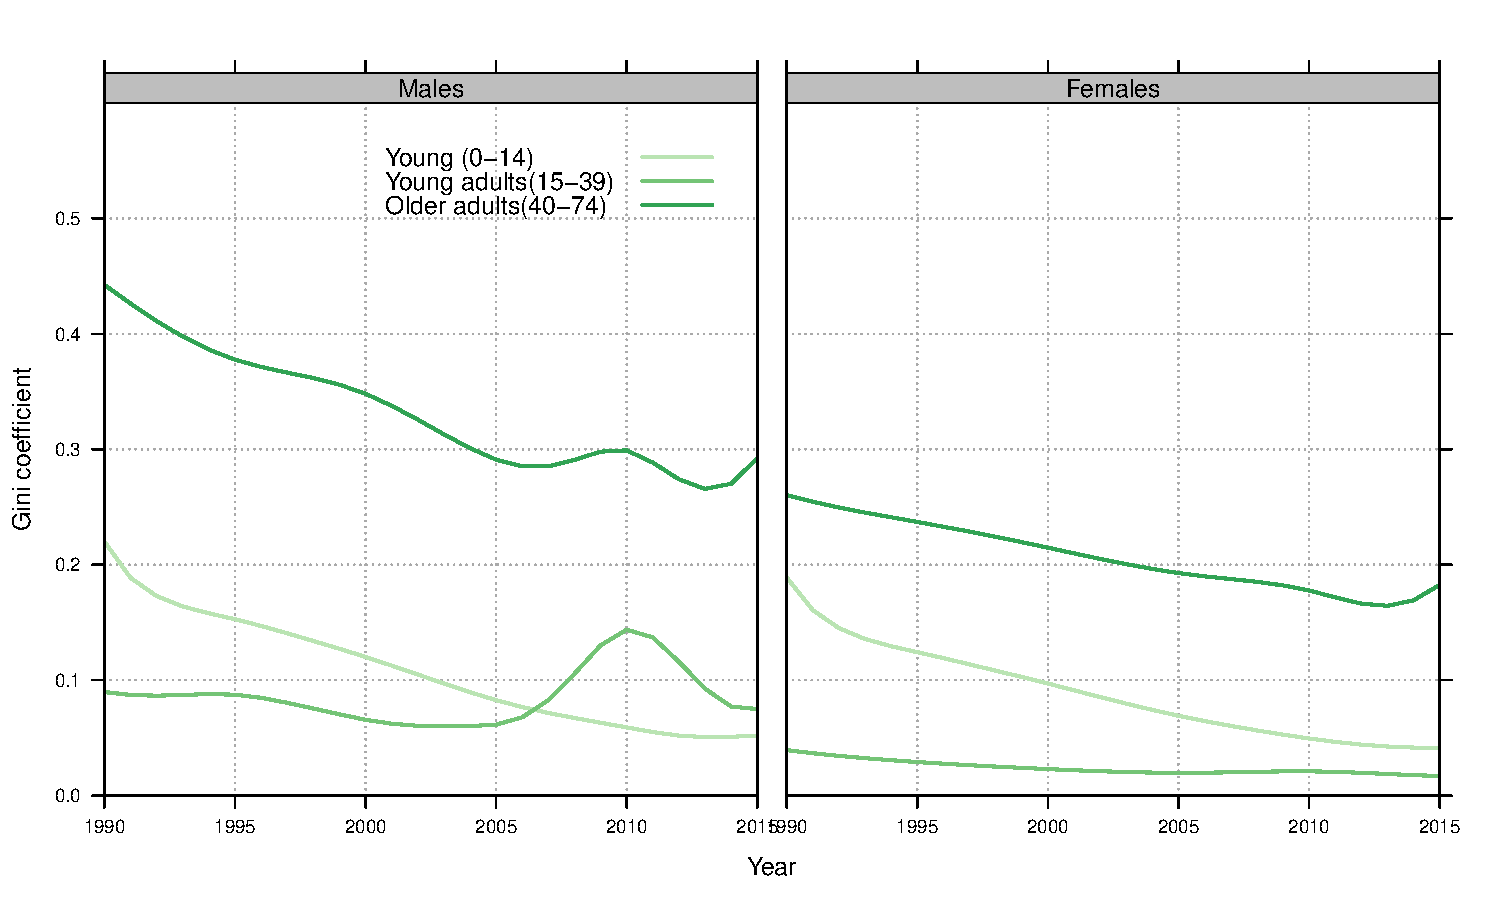
\includegraphics[scale=.5]{Gini_fig.pdf}
\end{figure}


\begin{figure}[h!]
\centering
\caption{Cause-specific contributions to state differences from low mortality benchmark for older female adults (ages 50-84), 1990-2015. States grouped into three regions.)}
\label{fig:e40_74_females}
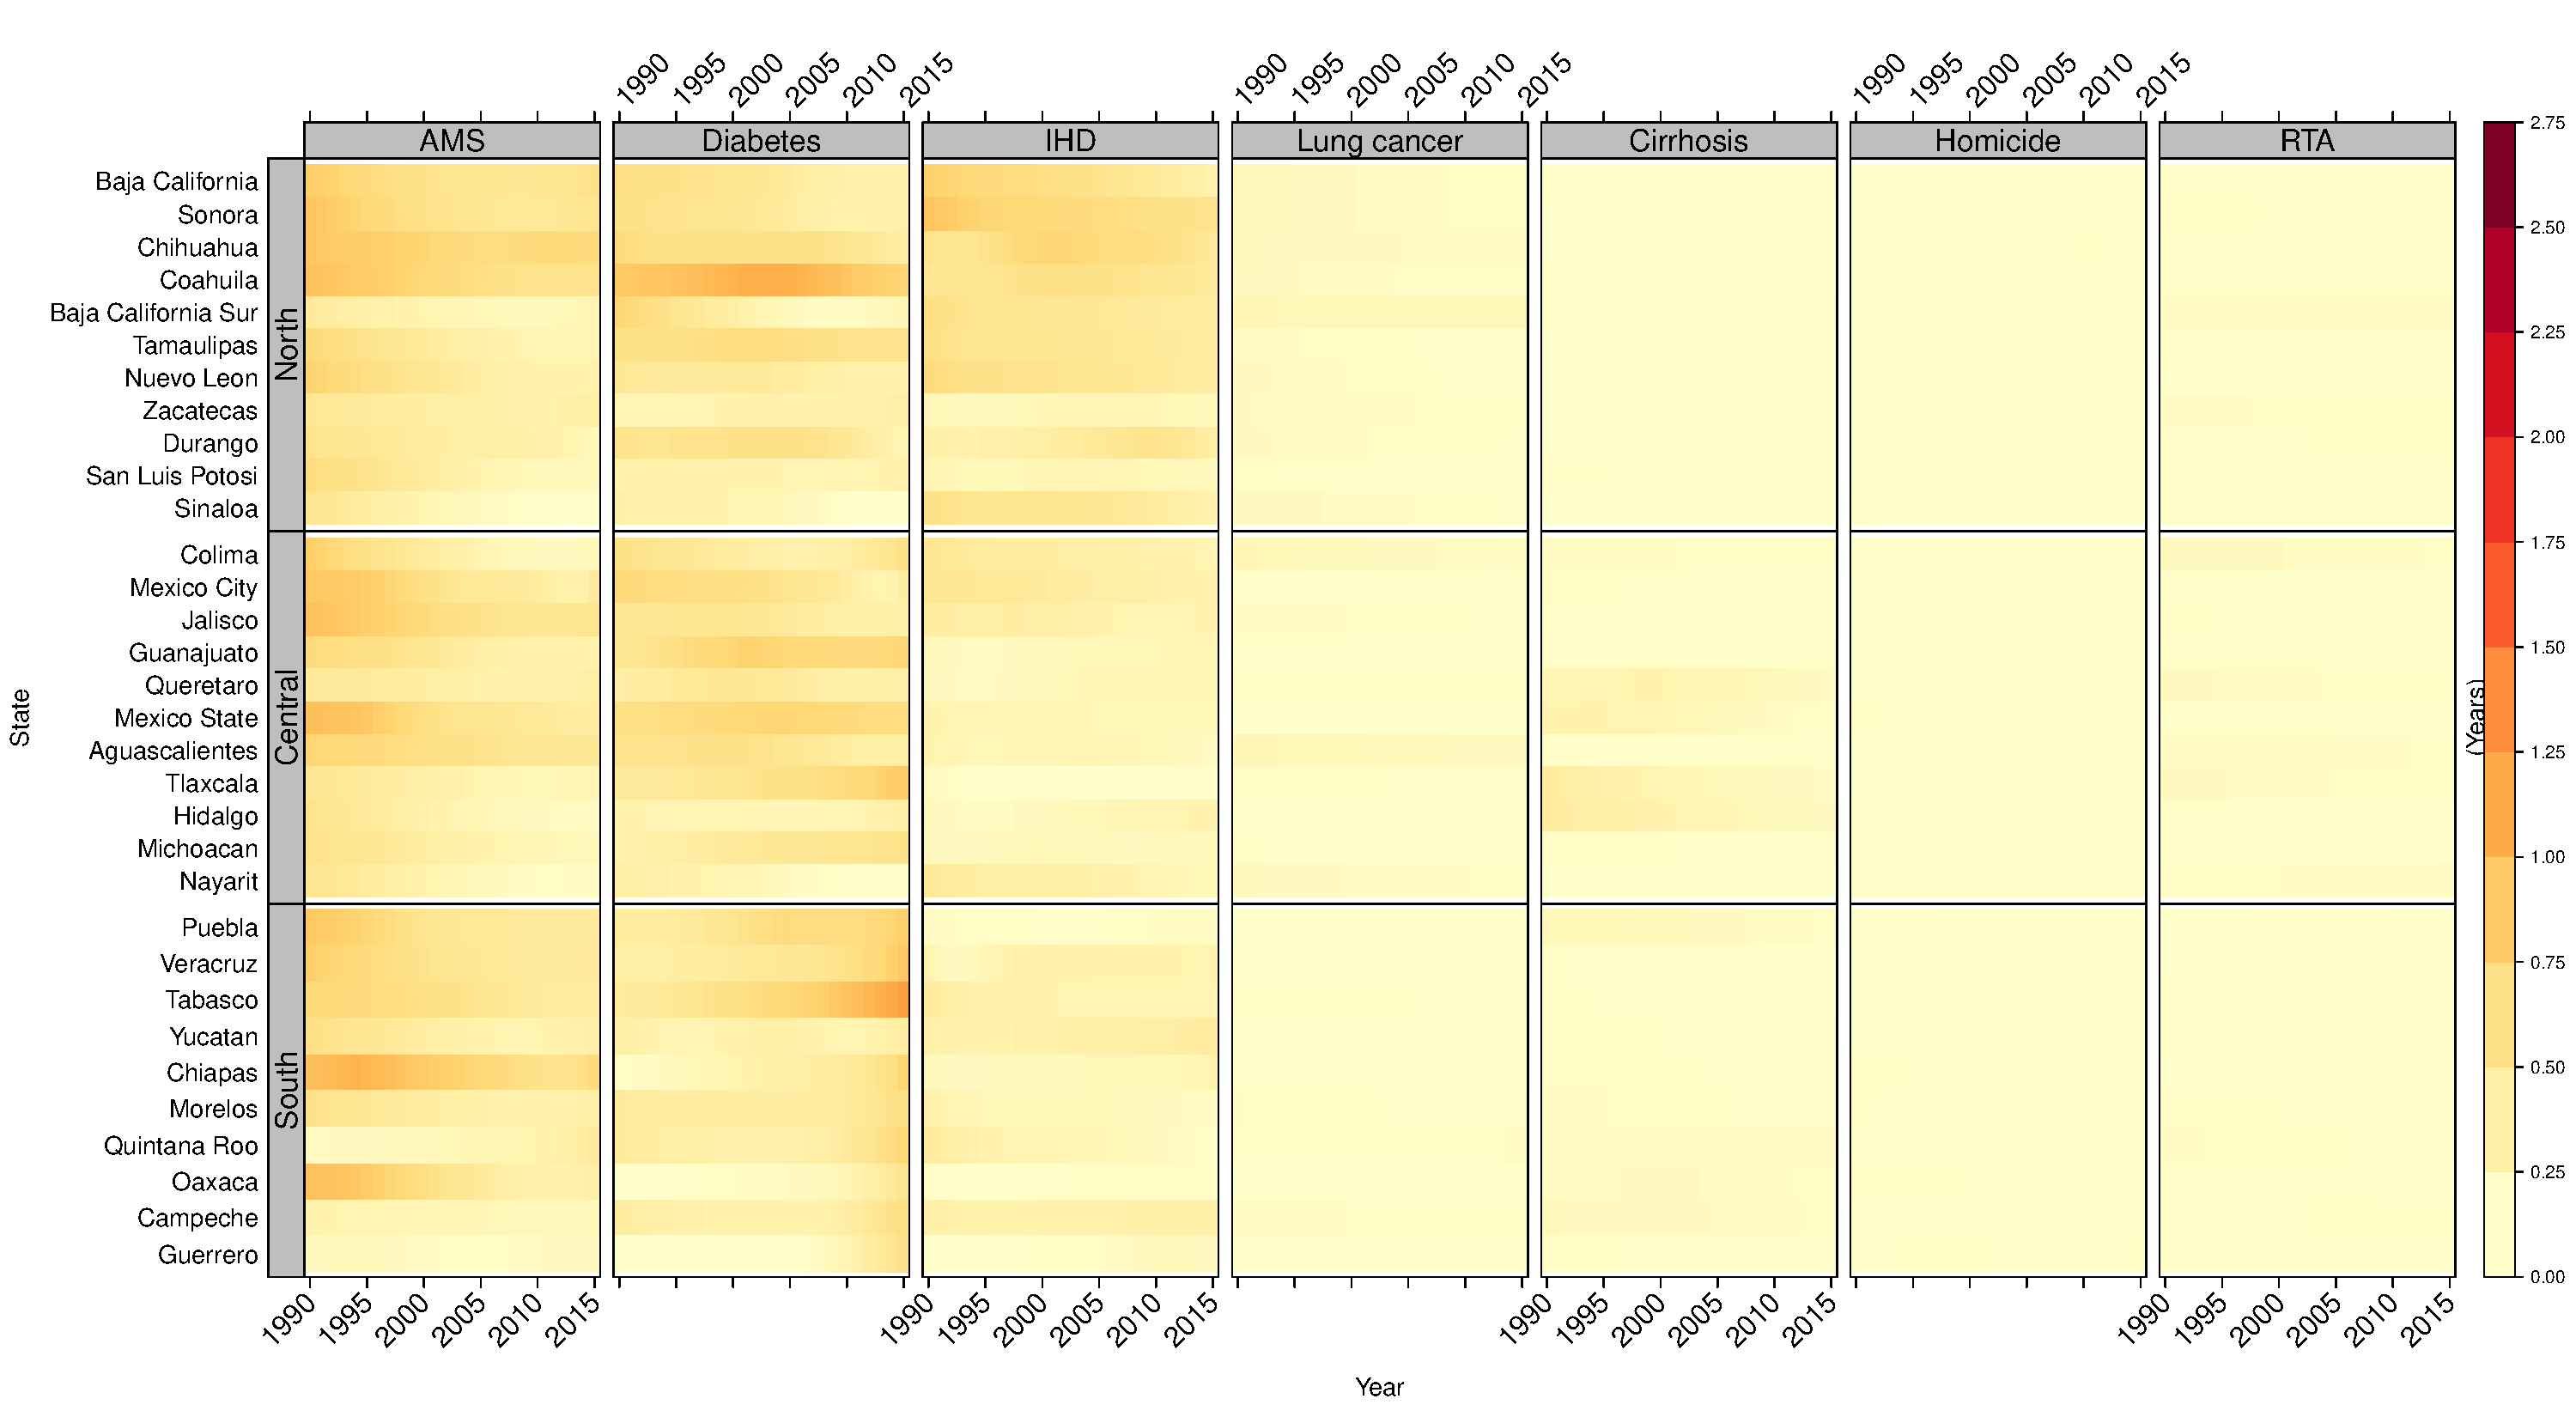
\includegraphics[scale=.31]{Adult_Female_heatmap.pdf}
Note: AMS is ``amenable to medical service'', IHD is ``isquemic heart diseases'', and RTA is ``road traffic accidents''. Source: own elaborations. \end{figure}


\begin{figure}
\centering
\caption{Cause-specific contributions to state differences from low mortality benchmark for male young population (ages 0-14), 1990-2015.}
\label{fig:e0_14_males}
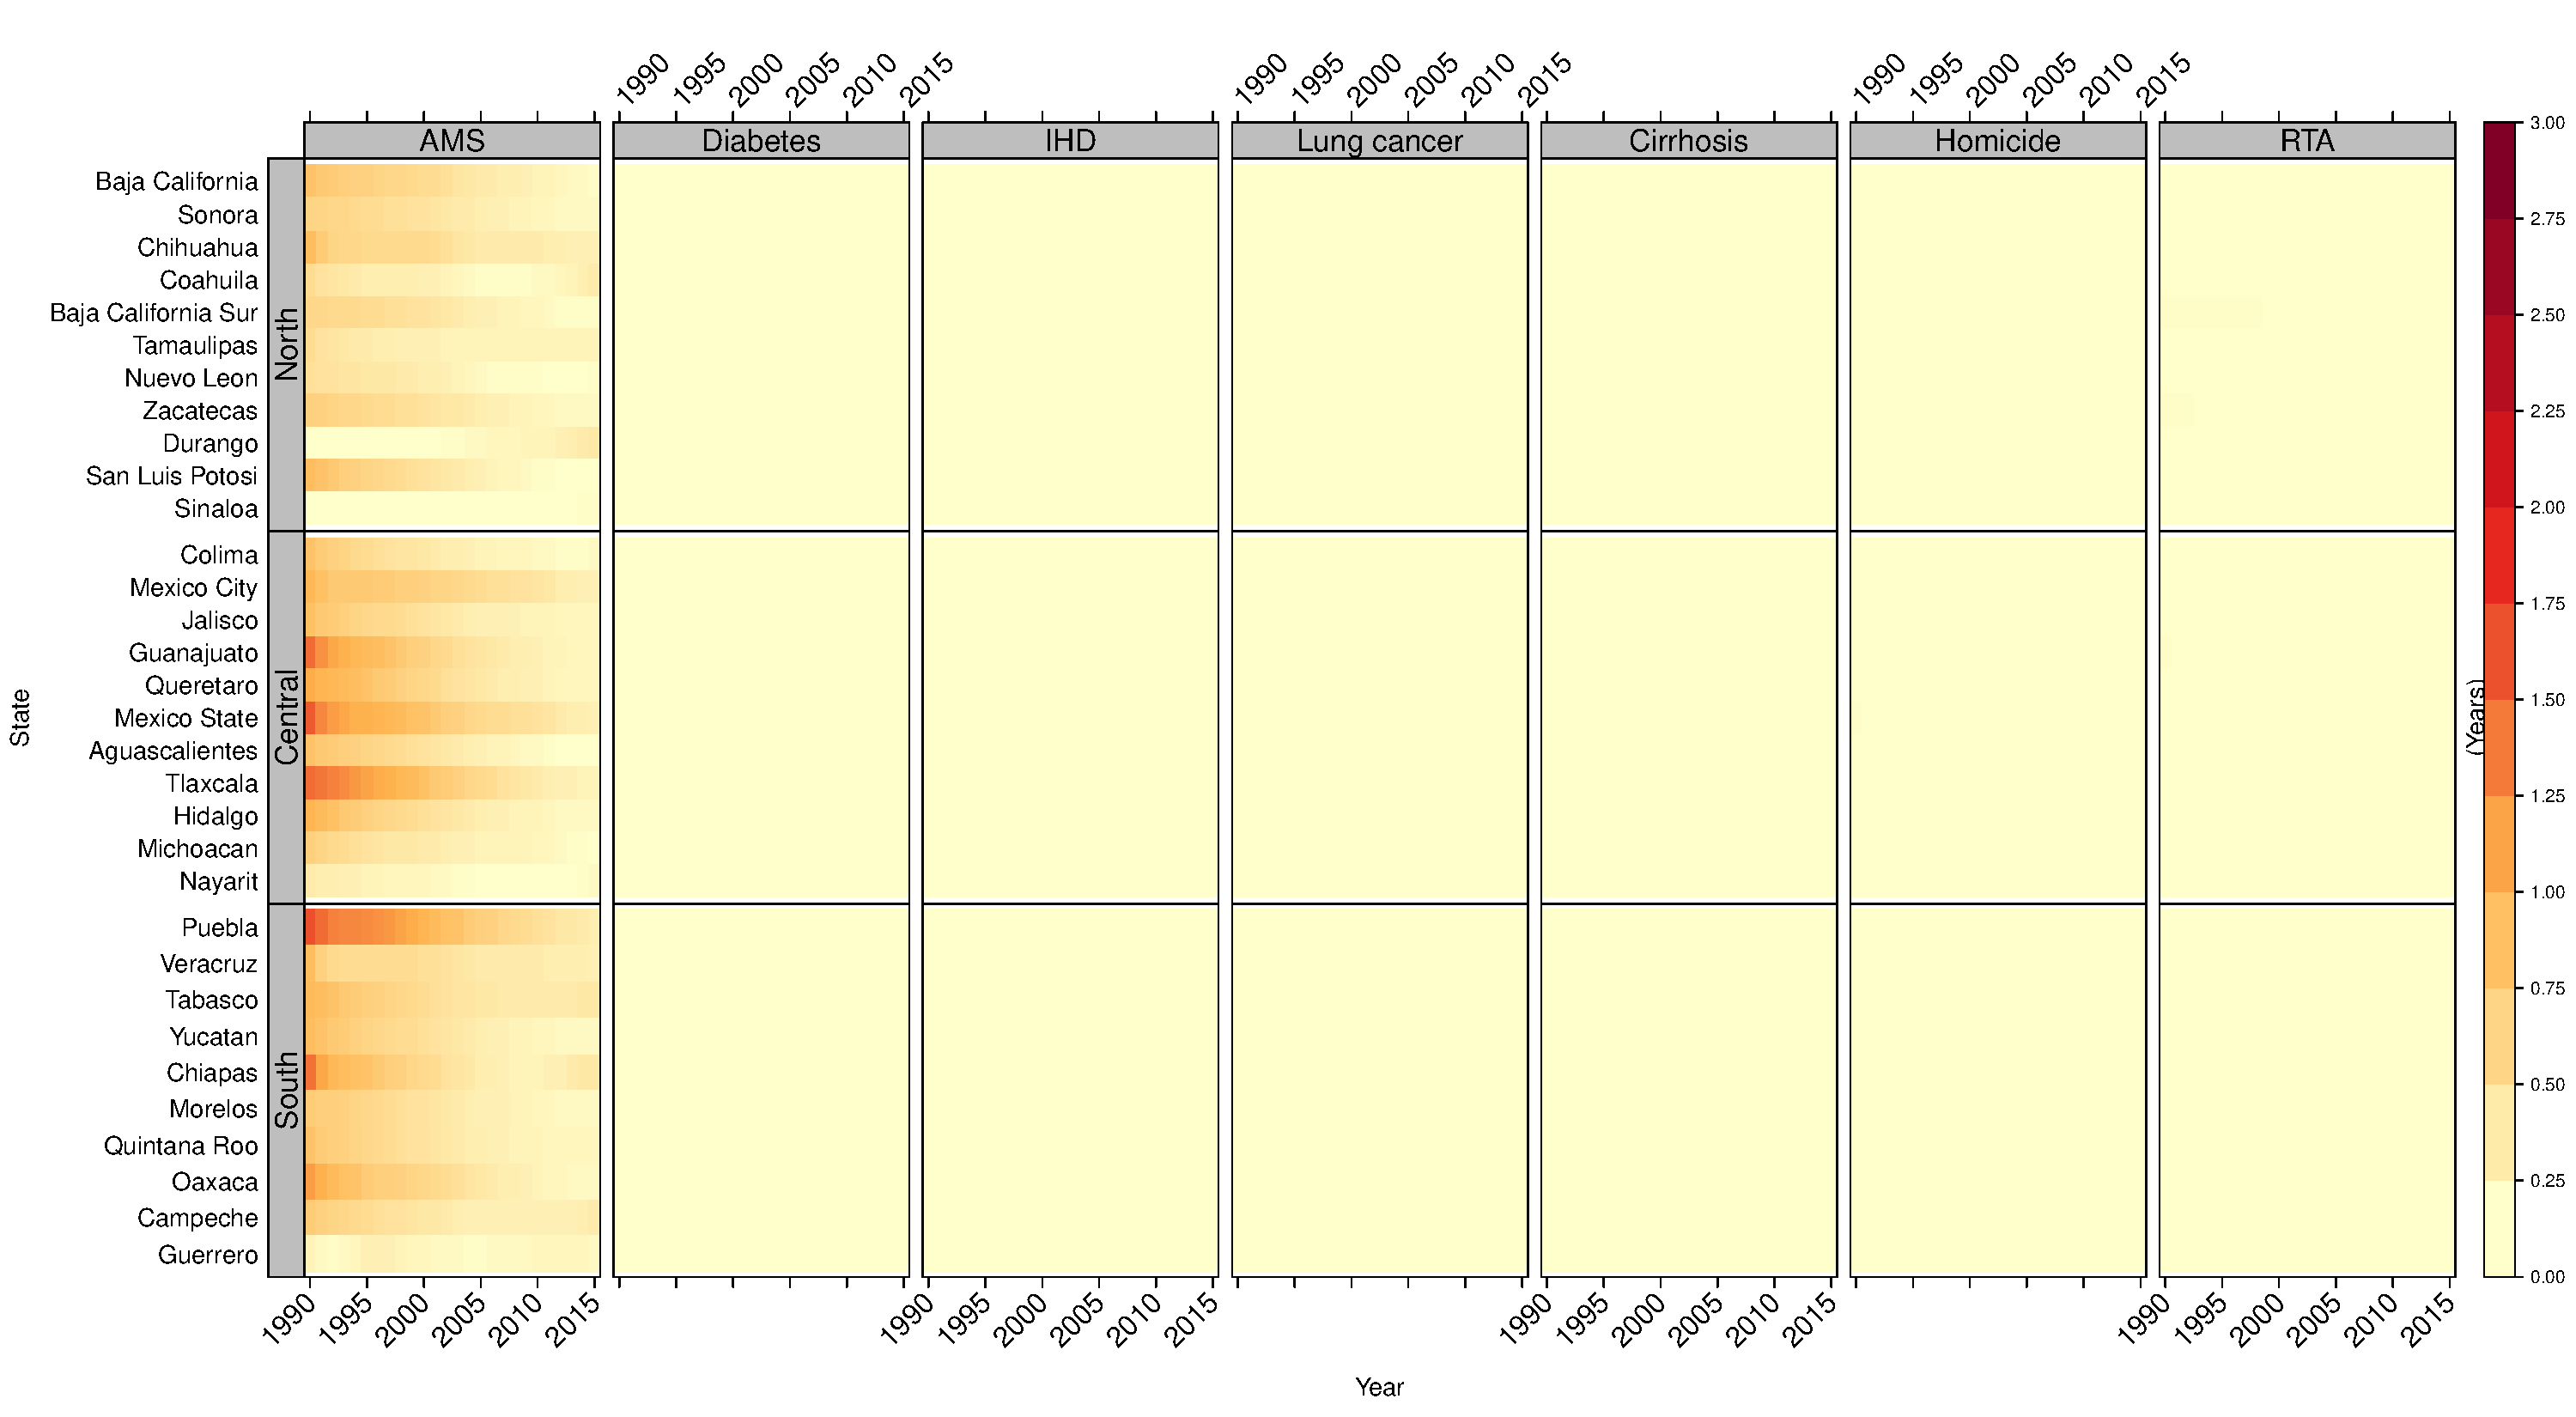
\includegraphics[scale=.3]{Young_Male_heatmap.pdf}
Note: AMS is ``amenable to medical service'', IHD is ``isquemic heart diseases'', and RTA is ``road traffic accidents''. Source: own elaborations.\end{figure}

\begin{figure}
\centering
\caption{Cause-specific contributions to state differences from low mortality benchmark for female young population (ages 0-14), 1990-2015.}
\label{fig:e0_14_females}
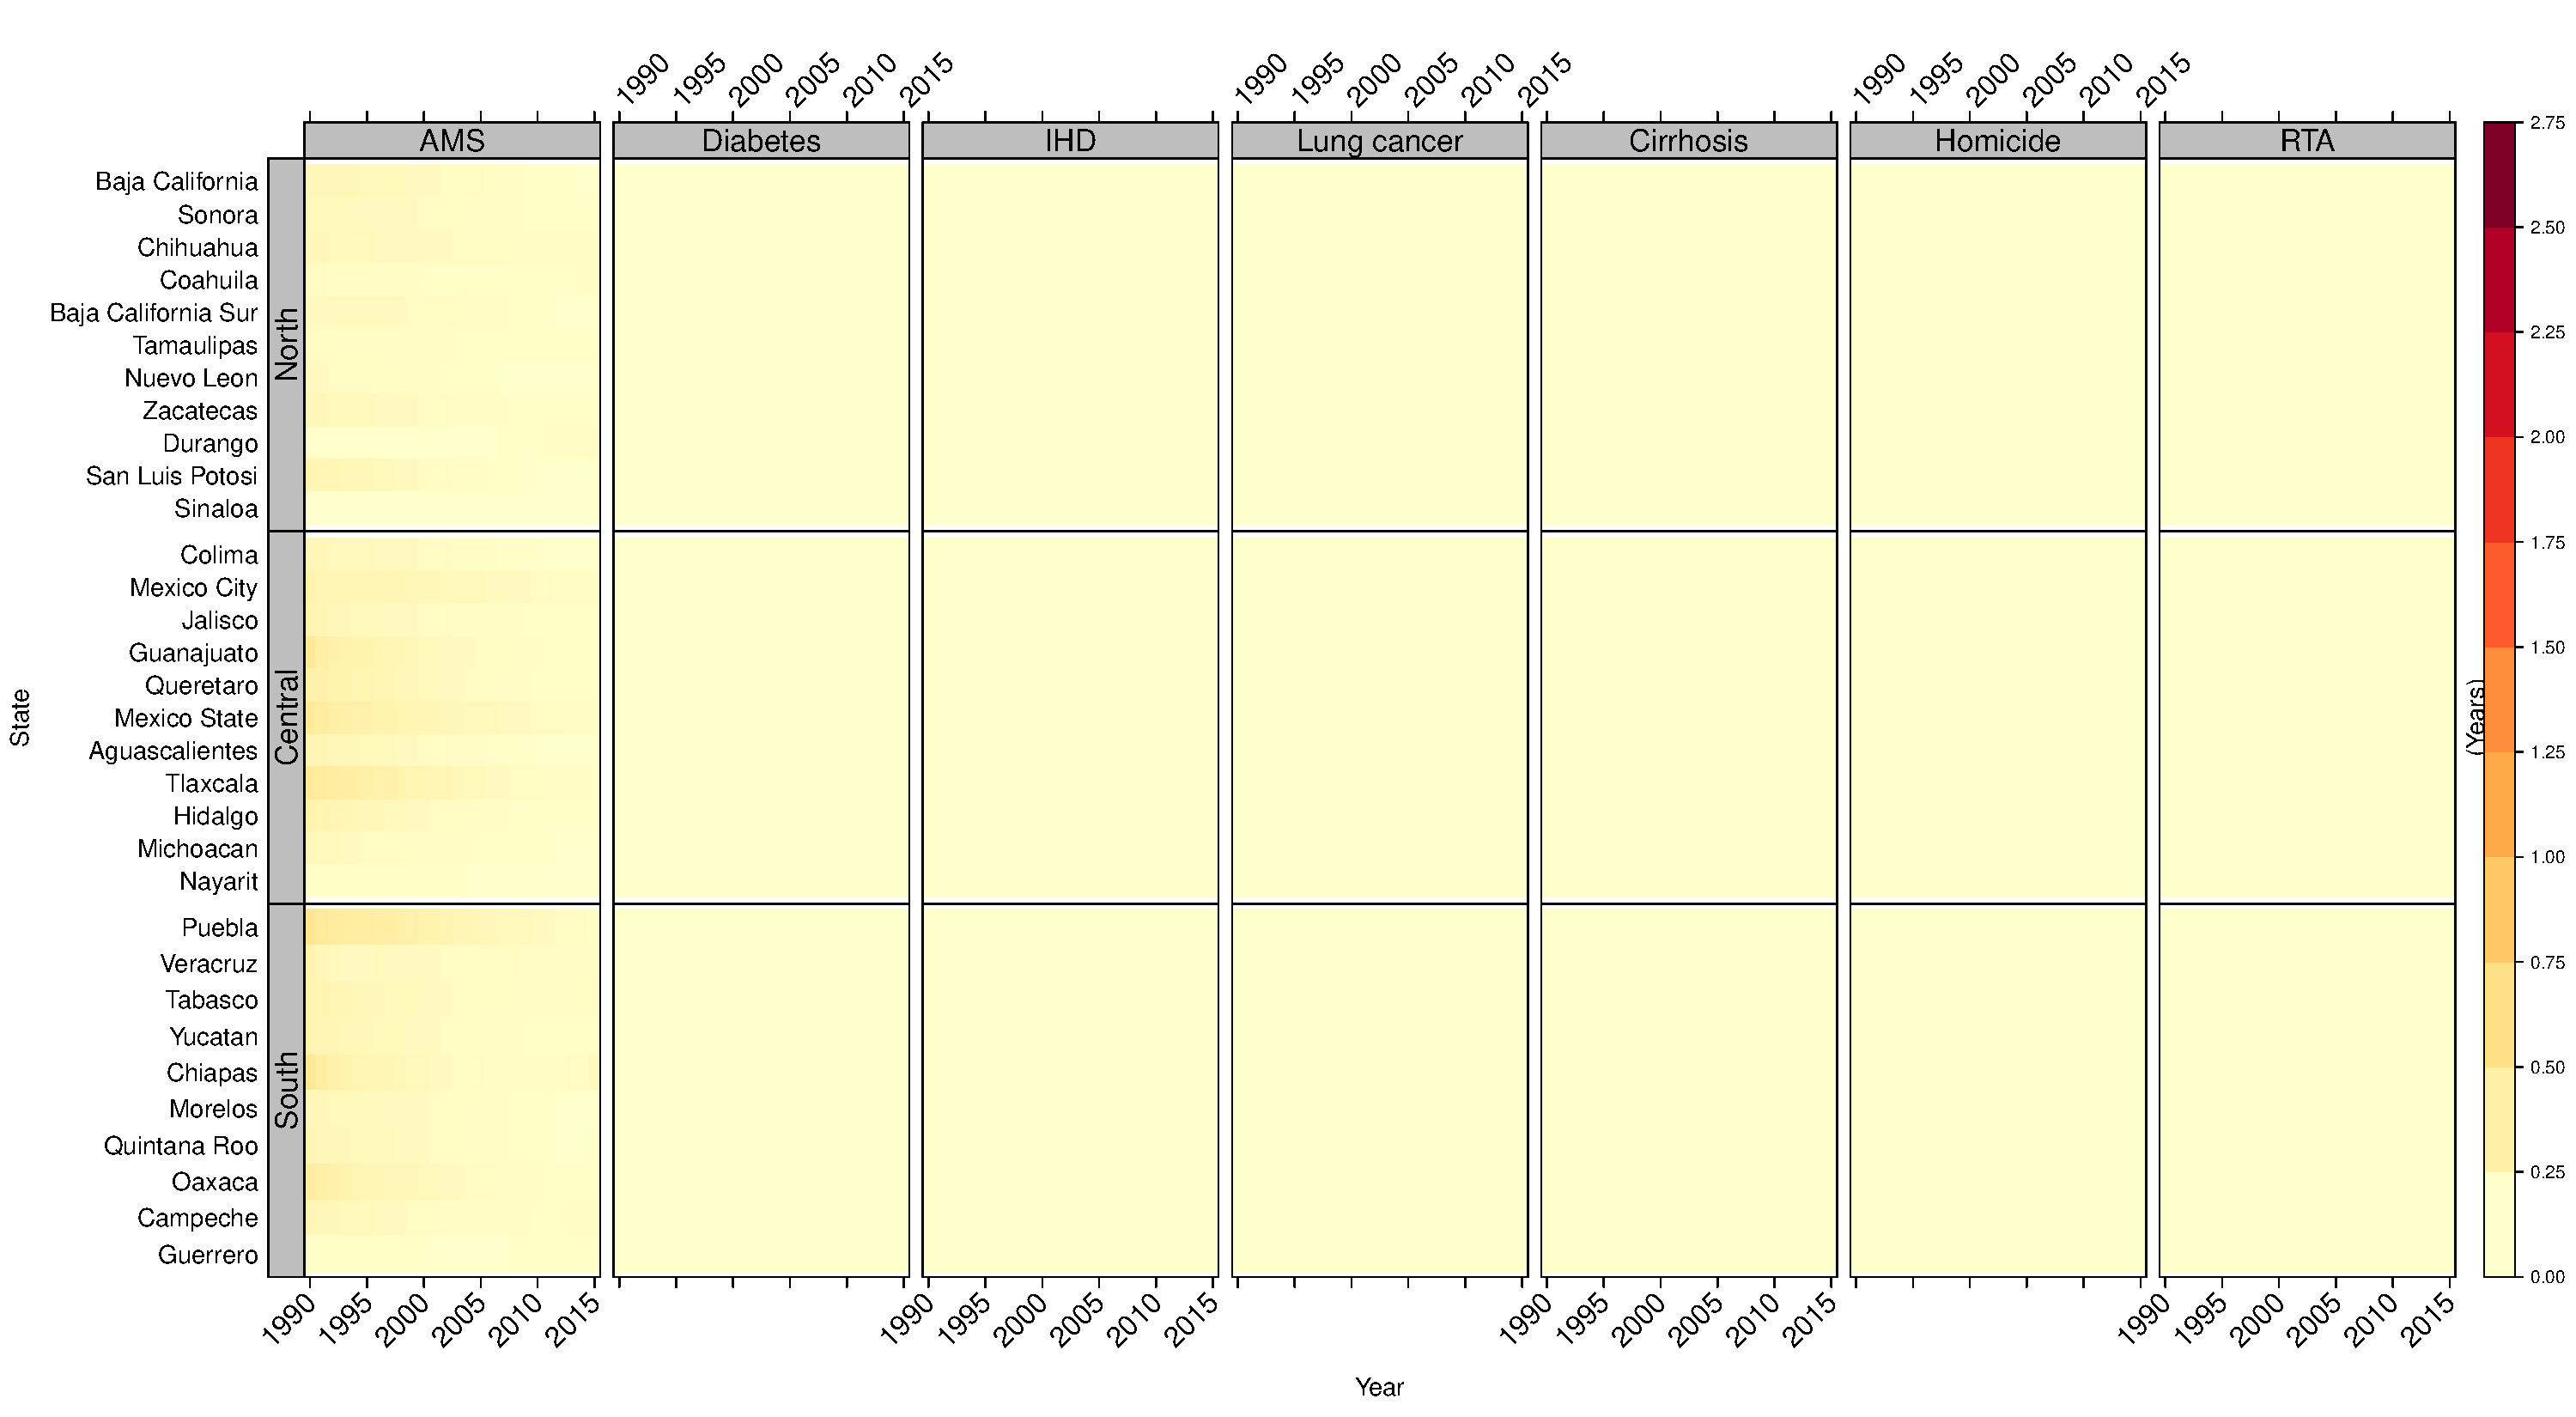
\includegraphics[scale=.3]{Young_Female_heatmap.pdf}
Note: AMS is ``amenable to medical service'', IHD is ``isquemic heart diseases'', and RTA is ``road traffic accidents''. Source: own elaborations.\end{figure}


\begin{figure}
\centering
\caption{Cause-specific contributions to state differences from low mortality benchmark for male young adults (ages 15-49), 1990-2015.}
\label{fig:e15_39_males}
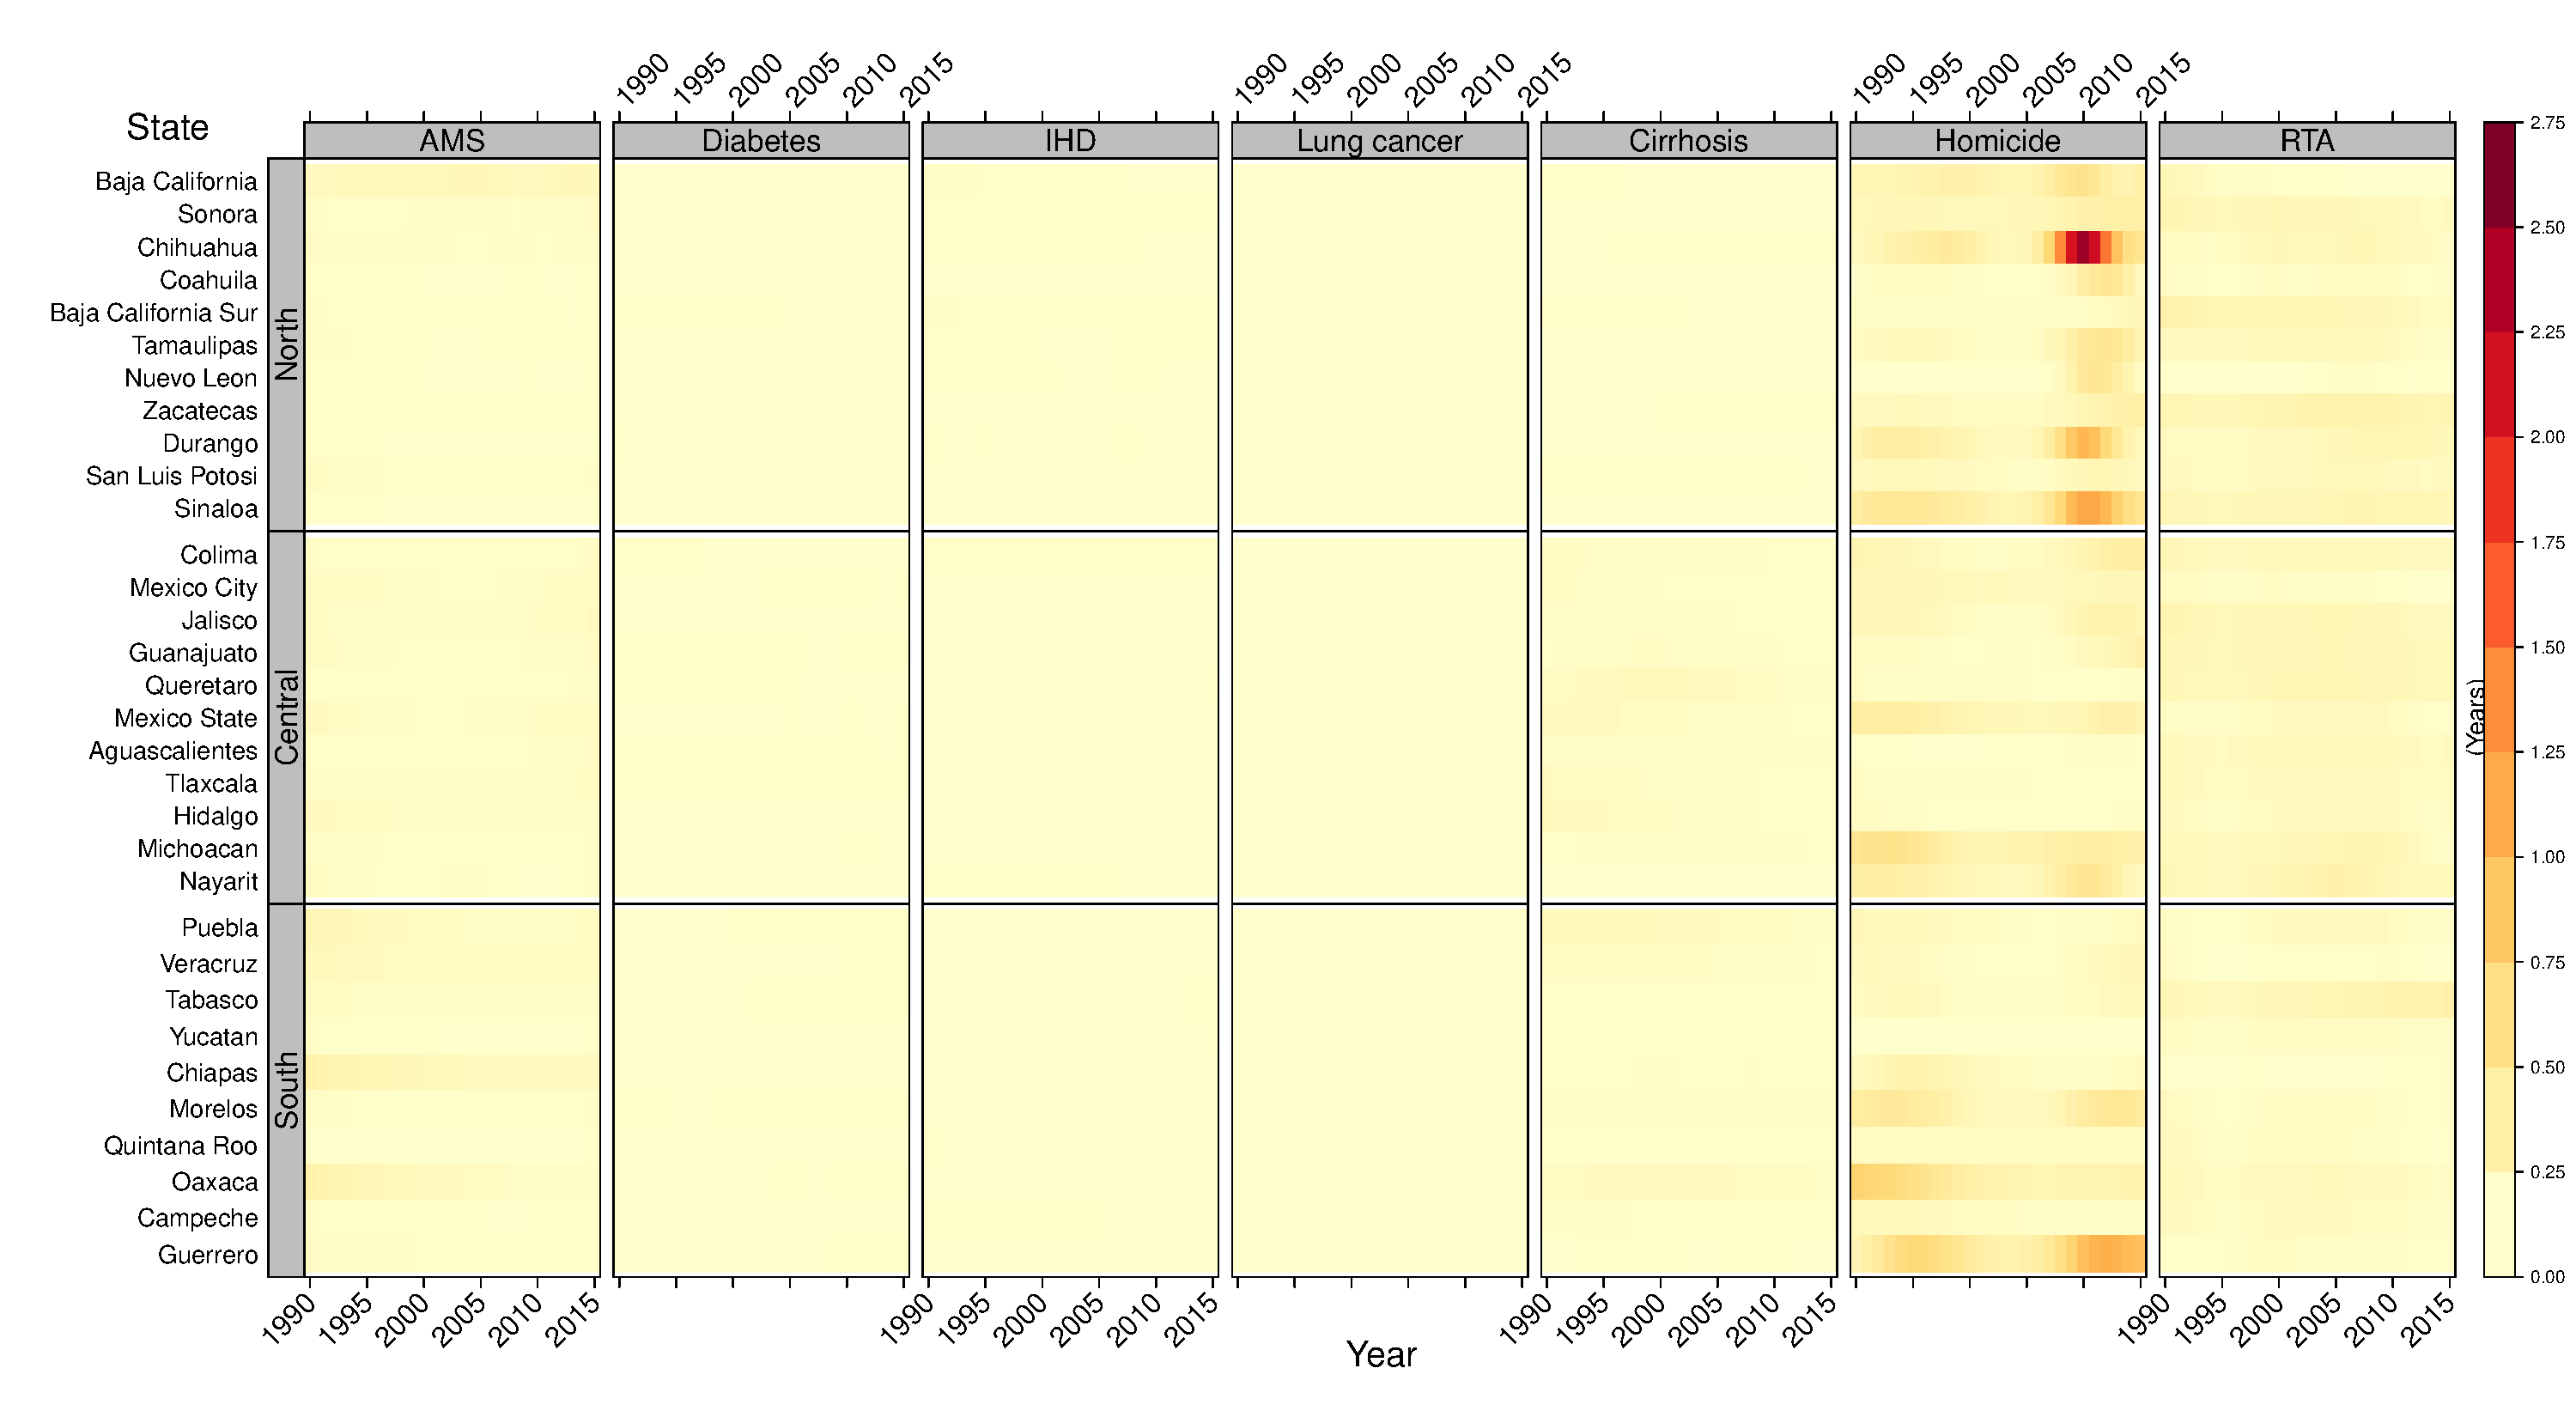
\includegraphics[scale=.3]{YoungAdult_Male_heatmap.pdf}
Note: AMS is ``amenable to medical service'', IHD is ``isquemic heart diseases'', and RTA is ``road traffic accidents''. Source: own elaborations.
\end{figure}

\begin{figure}
\centering
\caption{Cause-specific contributions to state differences from low mortality benchmark for female young adults (ages 15-49), 1990-2015.}
\label{fig:e15_39_females}
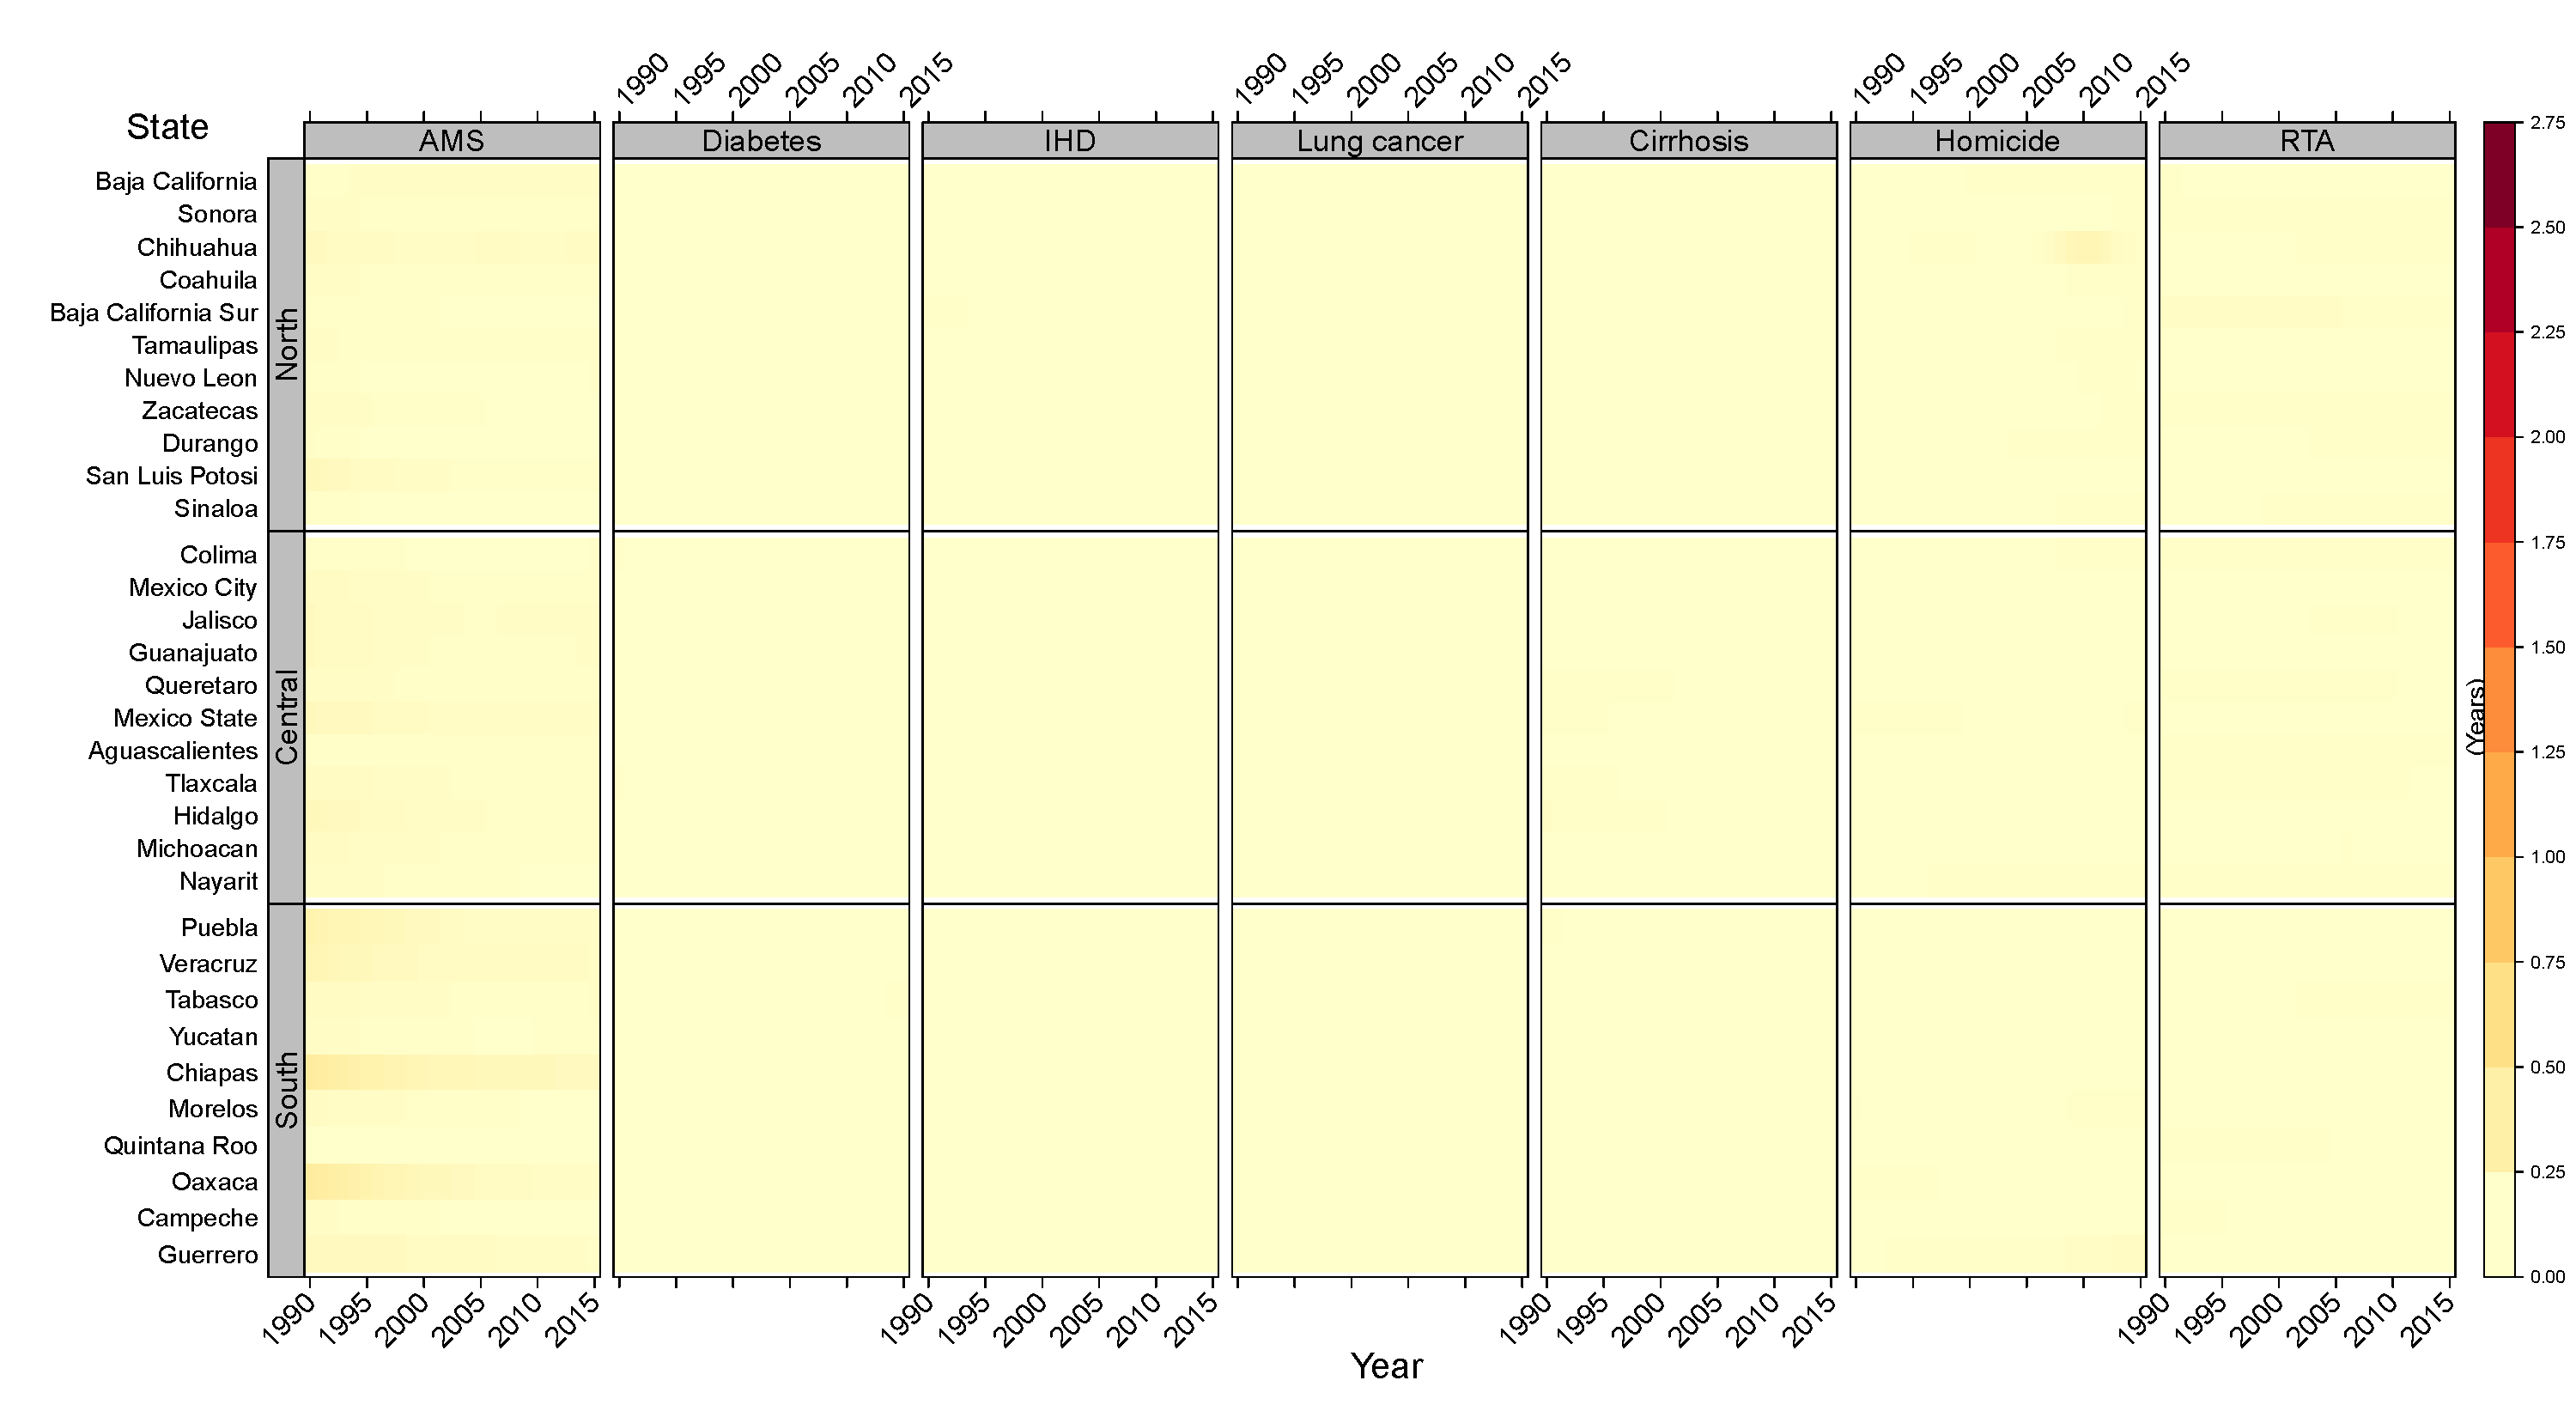
\includegraphics[scale=.3]{YoungAdult_Female_heatmap.pdf}
Note: AMS is ``amenable to medical service'', IHD is ``isquemic heart diseases'', and RTA is ``road traffic accidents''. Source: own elaborations.
\end{figure}



\begin{figure}
\centering
\caption{Distance from low mortality benchmark for selected years between ages 0-14. Source: own elaborations.}
\begin{center}
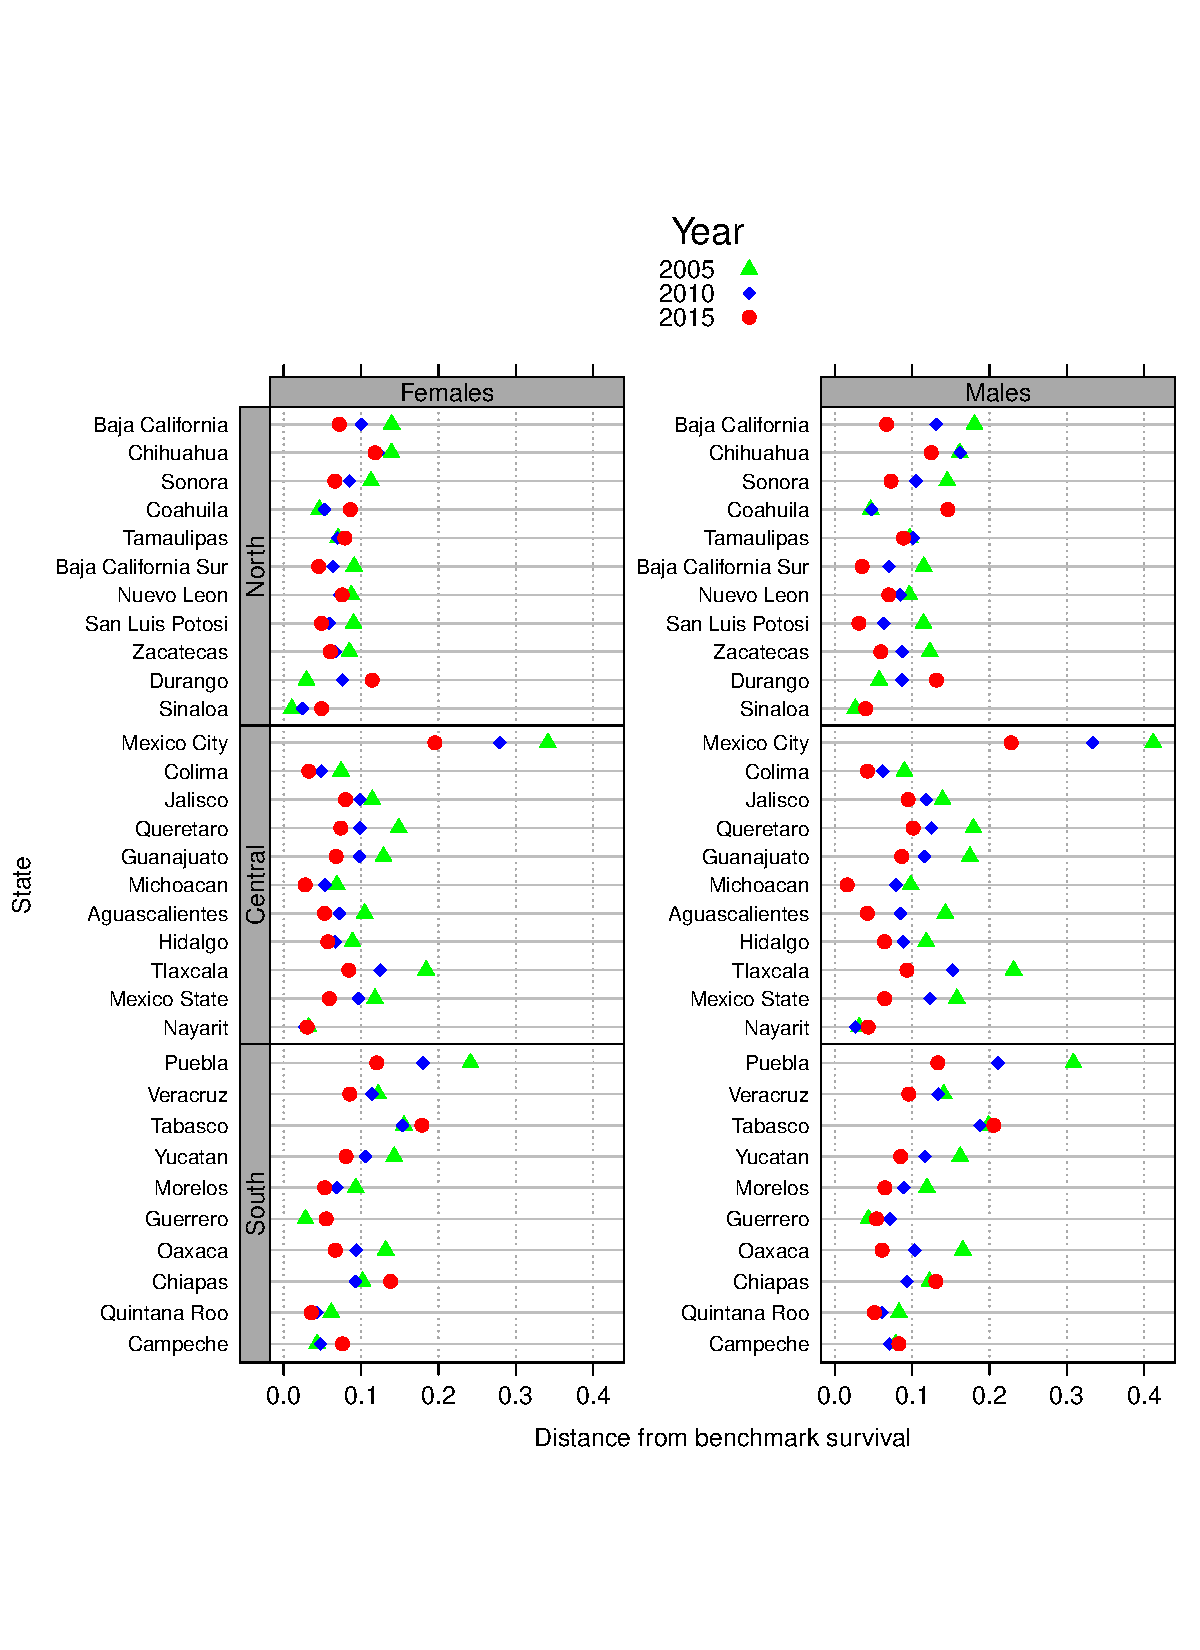
\includegraphics[scale=.5]{Distance_y.pdf}
\end{center}
\end{figure}

\begin{figure}
\centering
\caption{Distance from low mortality benchmark for selected years between ages 15-49. Source: own elaborations.}
\begin{center}
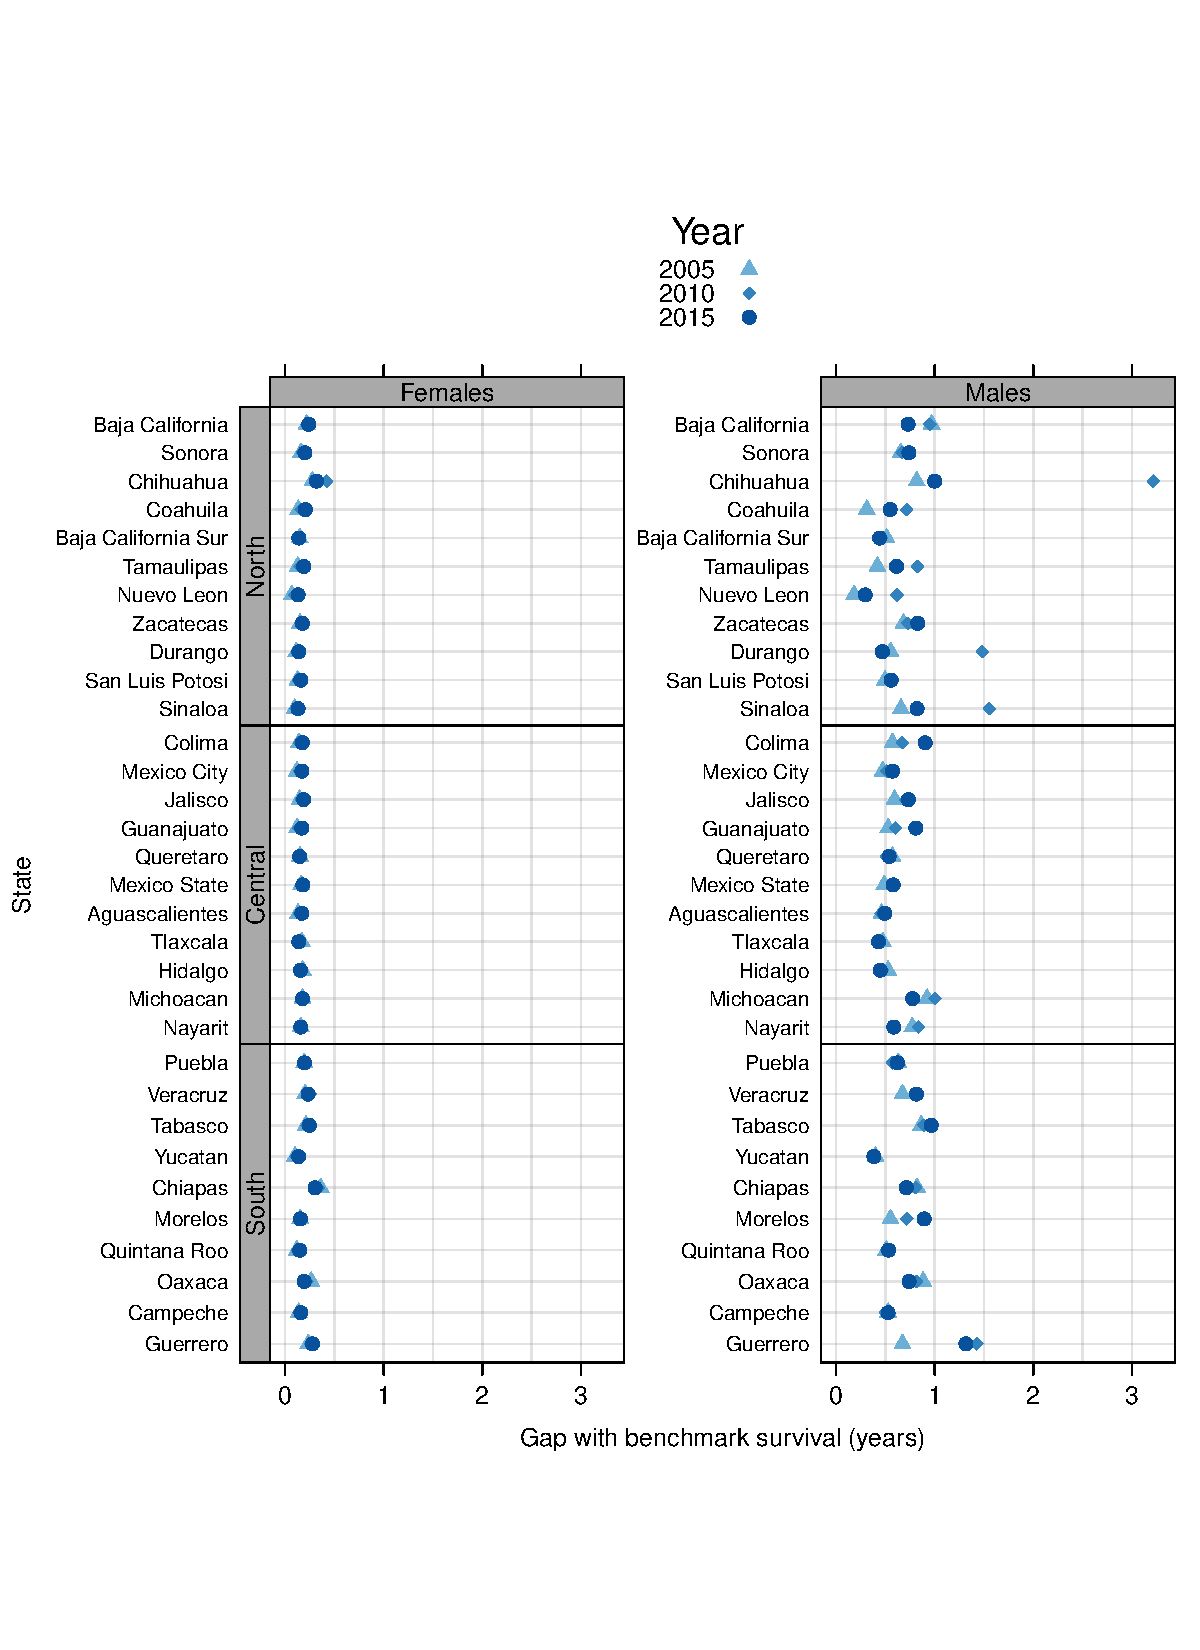
\includegraphics[scale=.5]{Distance_ya.pdf}
\end{center}
\end{figure}

\begin{figure}
\centering
\caption{Distance from low mortality benchmark for selected years between ages 50-84. Source: own elaborations.}
\begin{center}
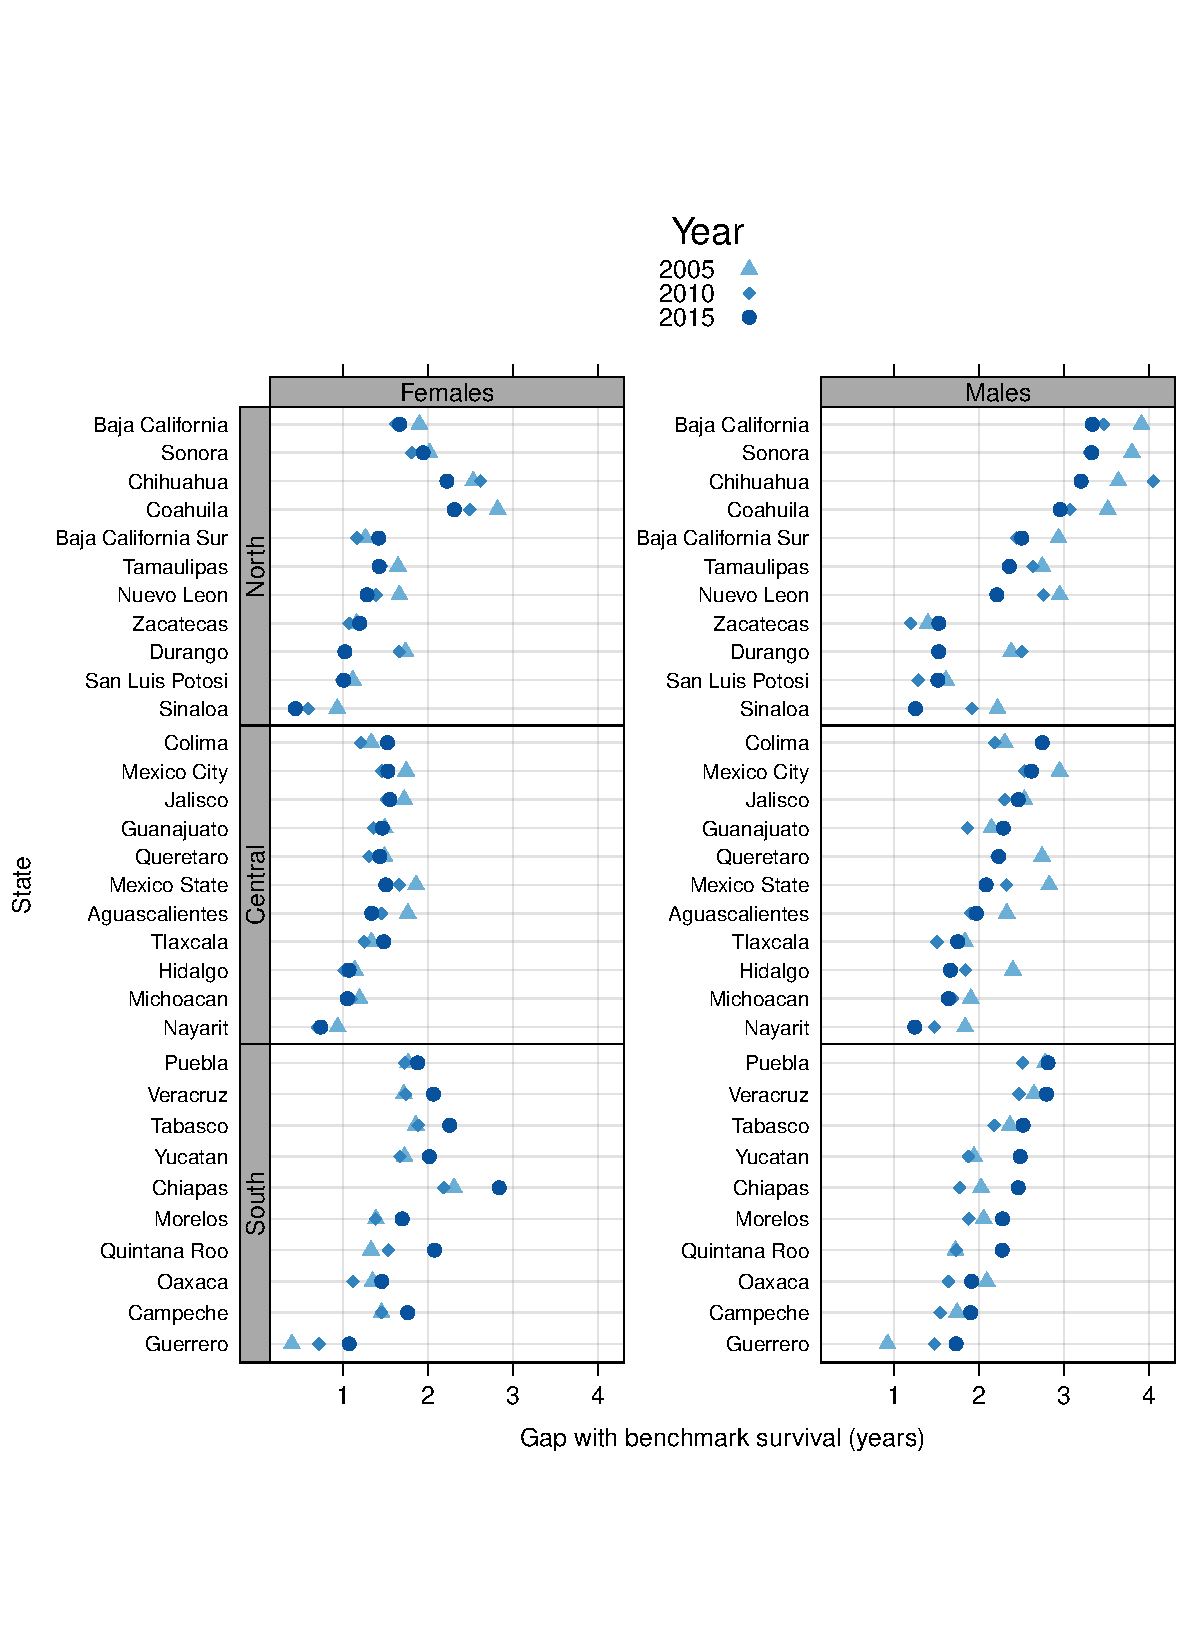
\includegraphics[scale=.5]{Distance_oa.pdf}
\end{center}
\end{figure}






\begin{figure}
\centering
\caption{Proportion by cause of death from benchmark mortality for young females (ages 0-14). Source: own elaborations.}
\begin{center}
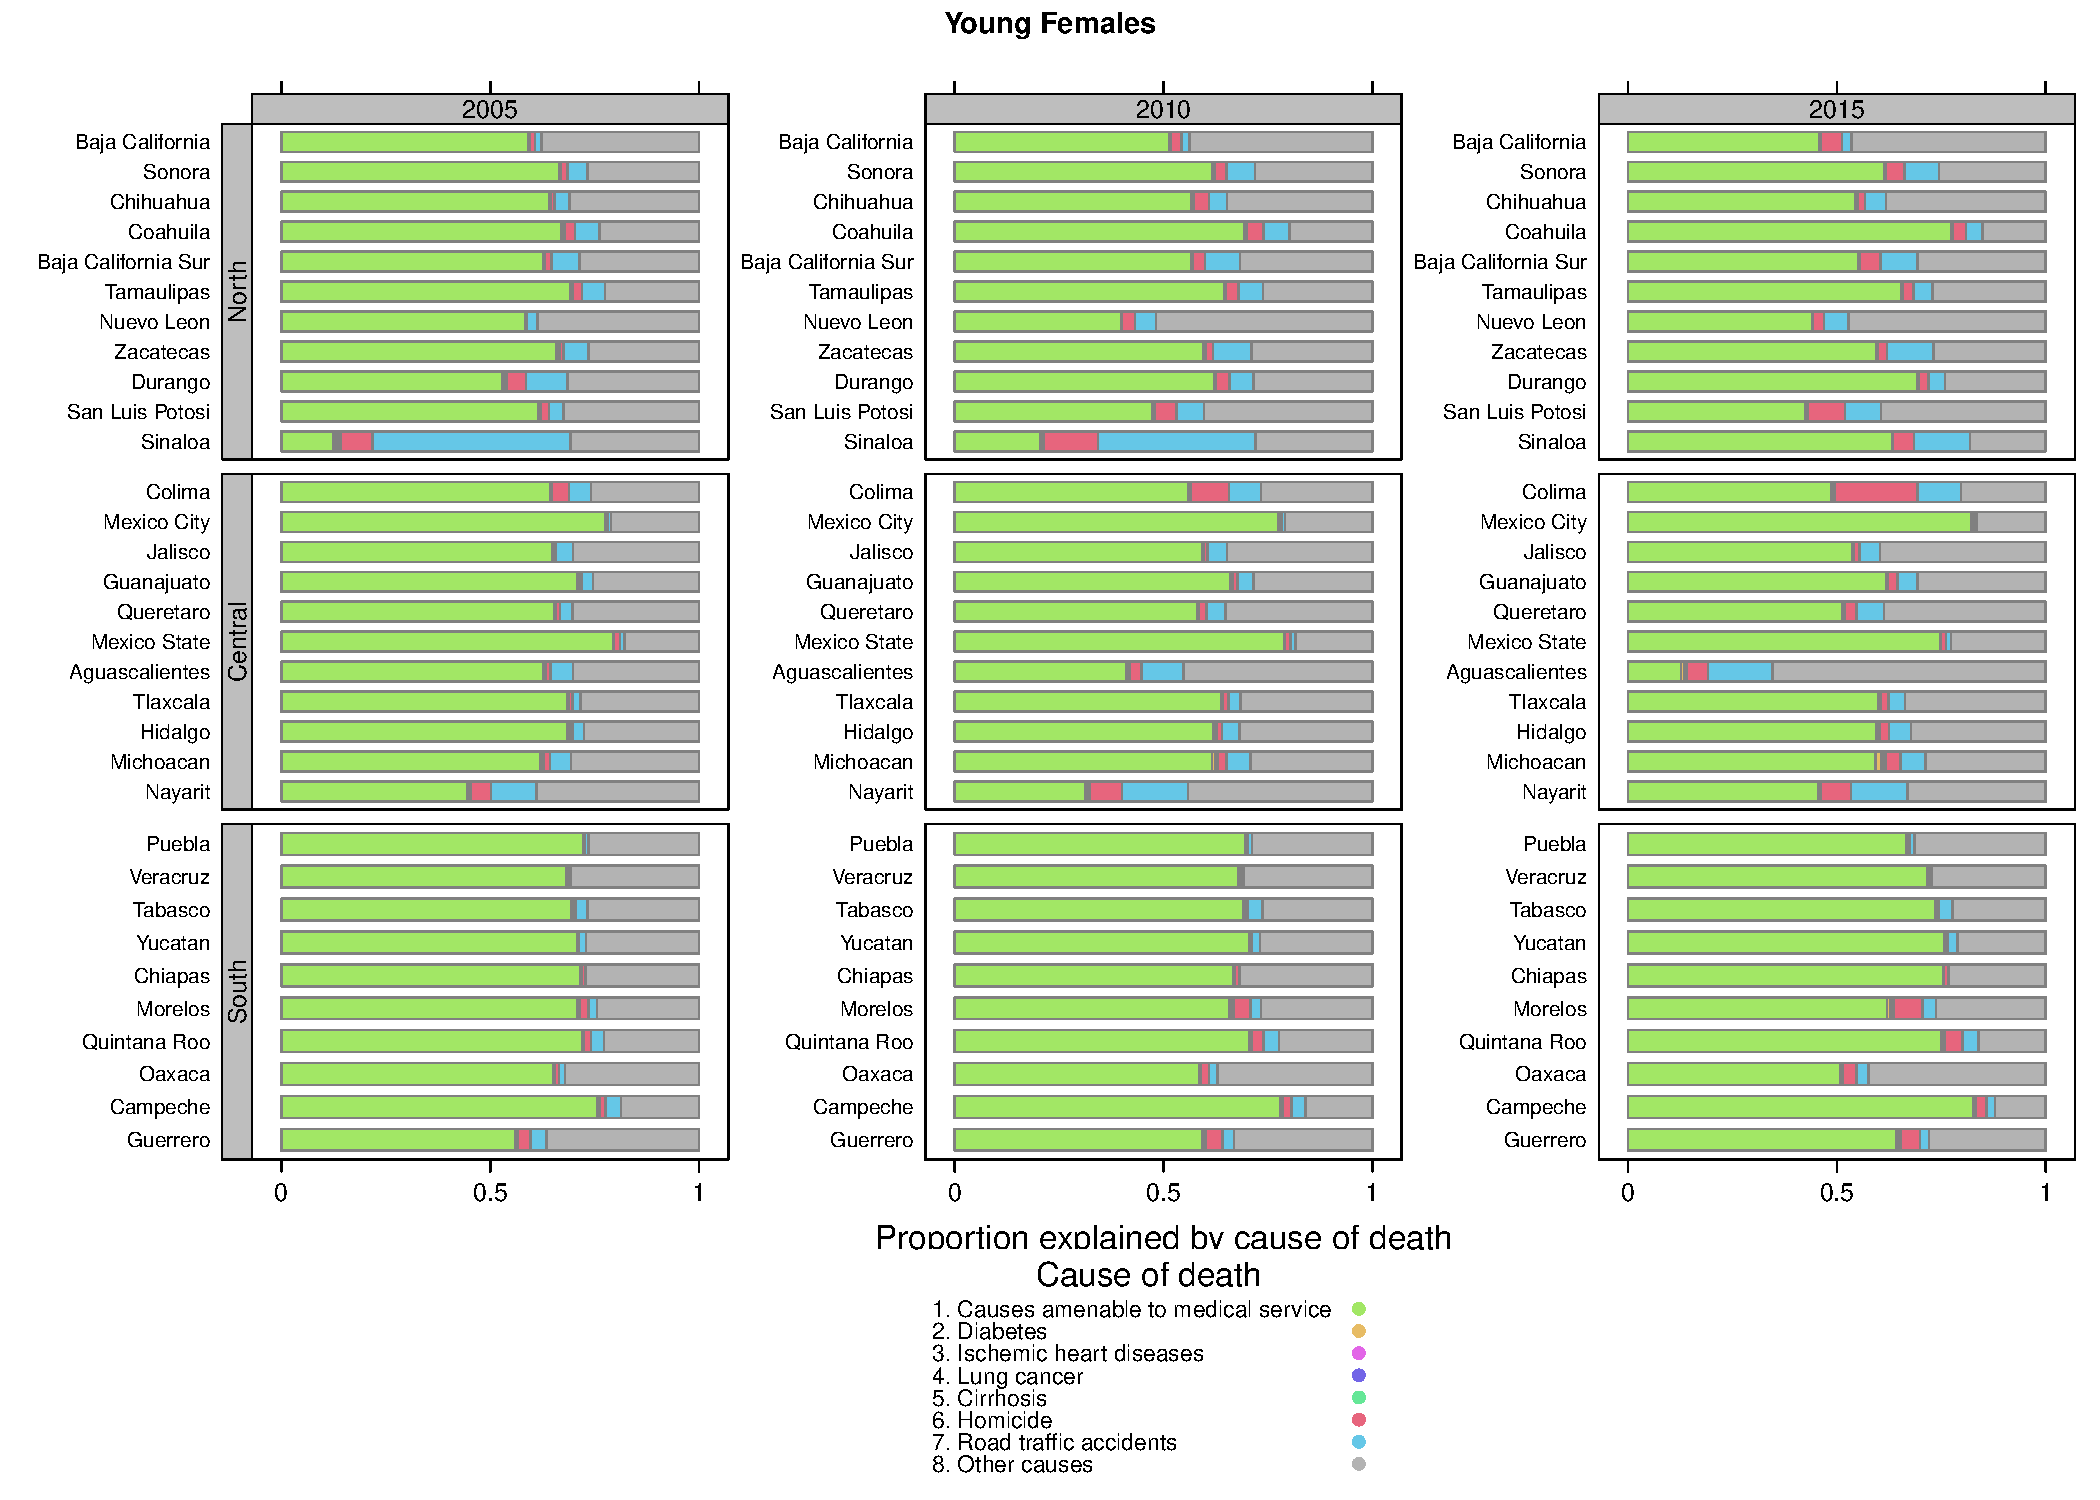
\includegraphics[scale=.45]{Figure_prop_yf.pdf}
\end{center}
\end{figure}

\begin{figure}
\centering
\caption{Proportion by cause of death from benchmark mortality for young males (ages 0-14). Source: own elaborations.}
\begin{center}
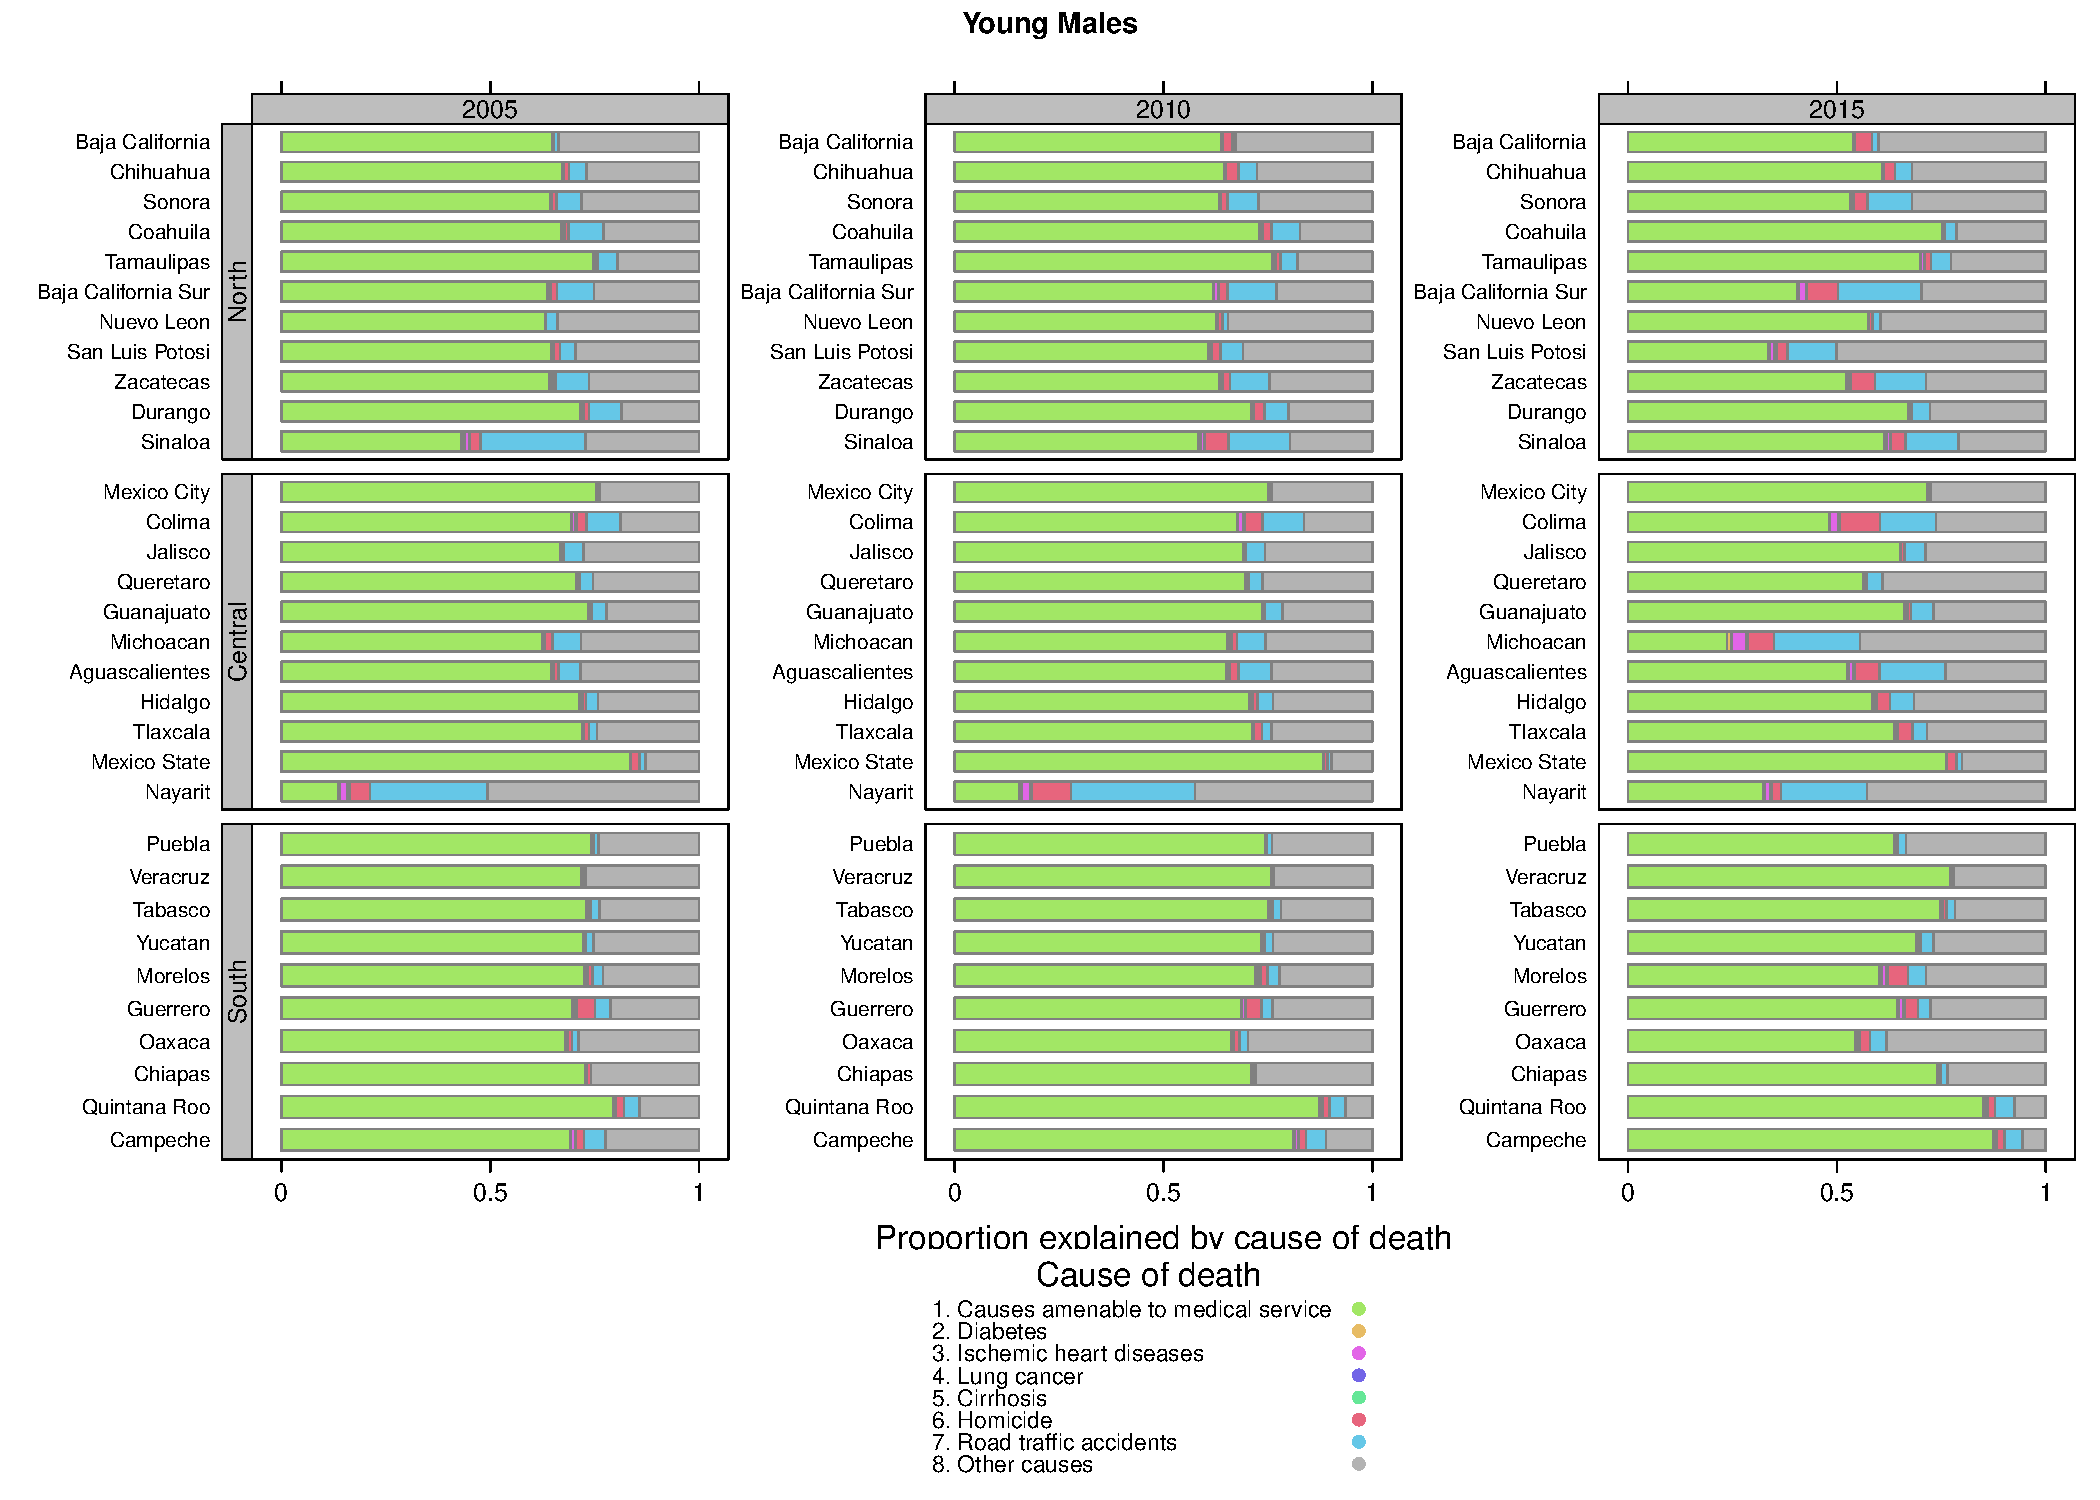
\includegraphics[scale=.45]{Figure_prop_ym.pdf}
\end{center}
\end{figure}



\begin{figure}
\centering
\caption{Proportion by cause of death from benchmark mortality for young adult females (ages 15-49). Source: own elaborations.}
\begin{center}
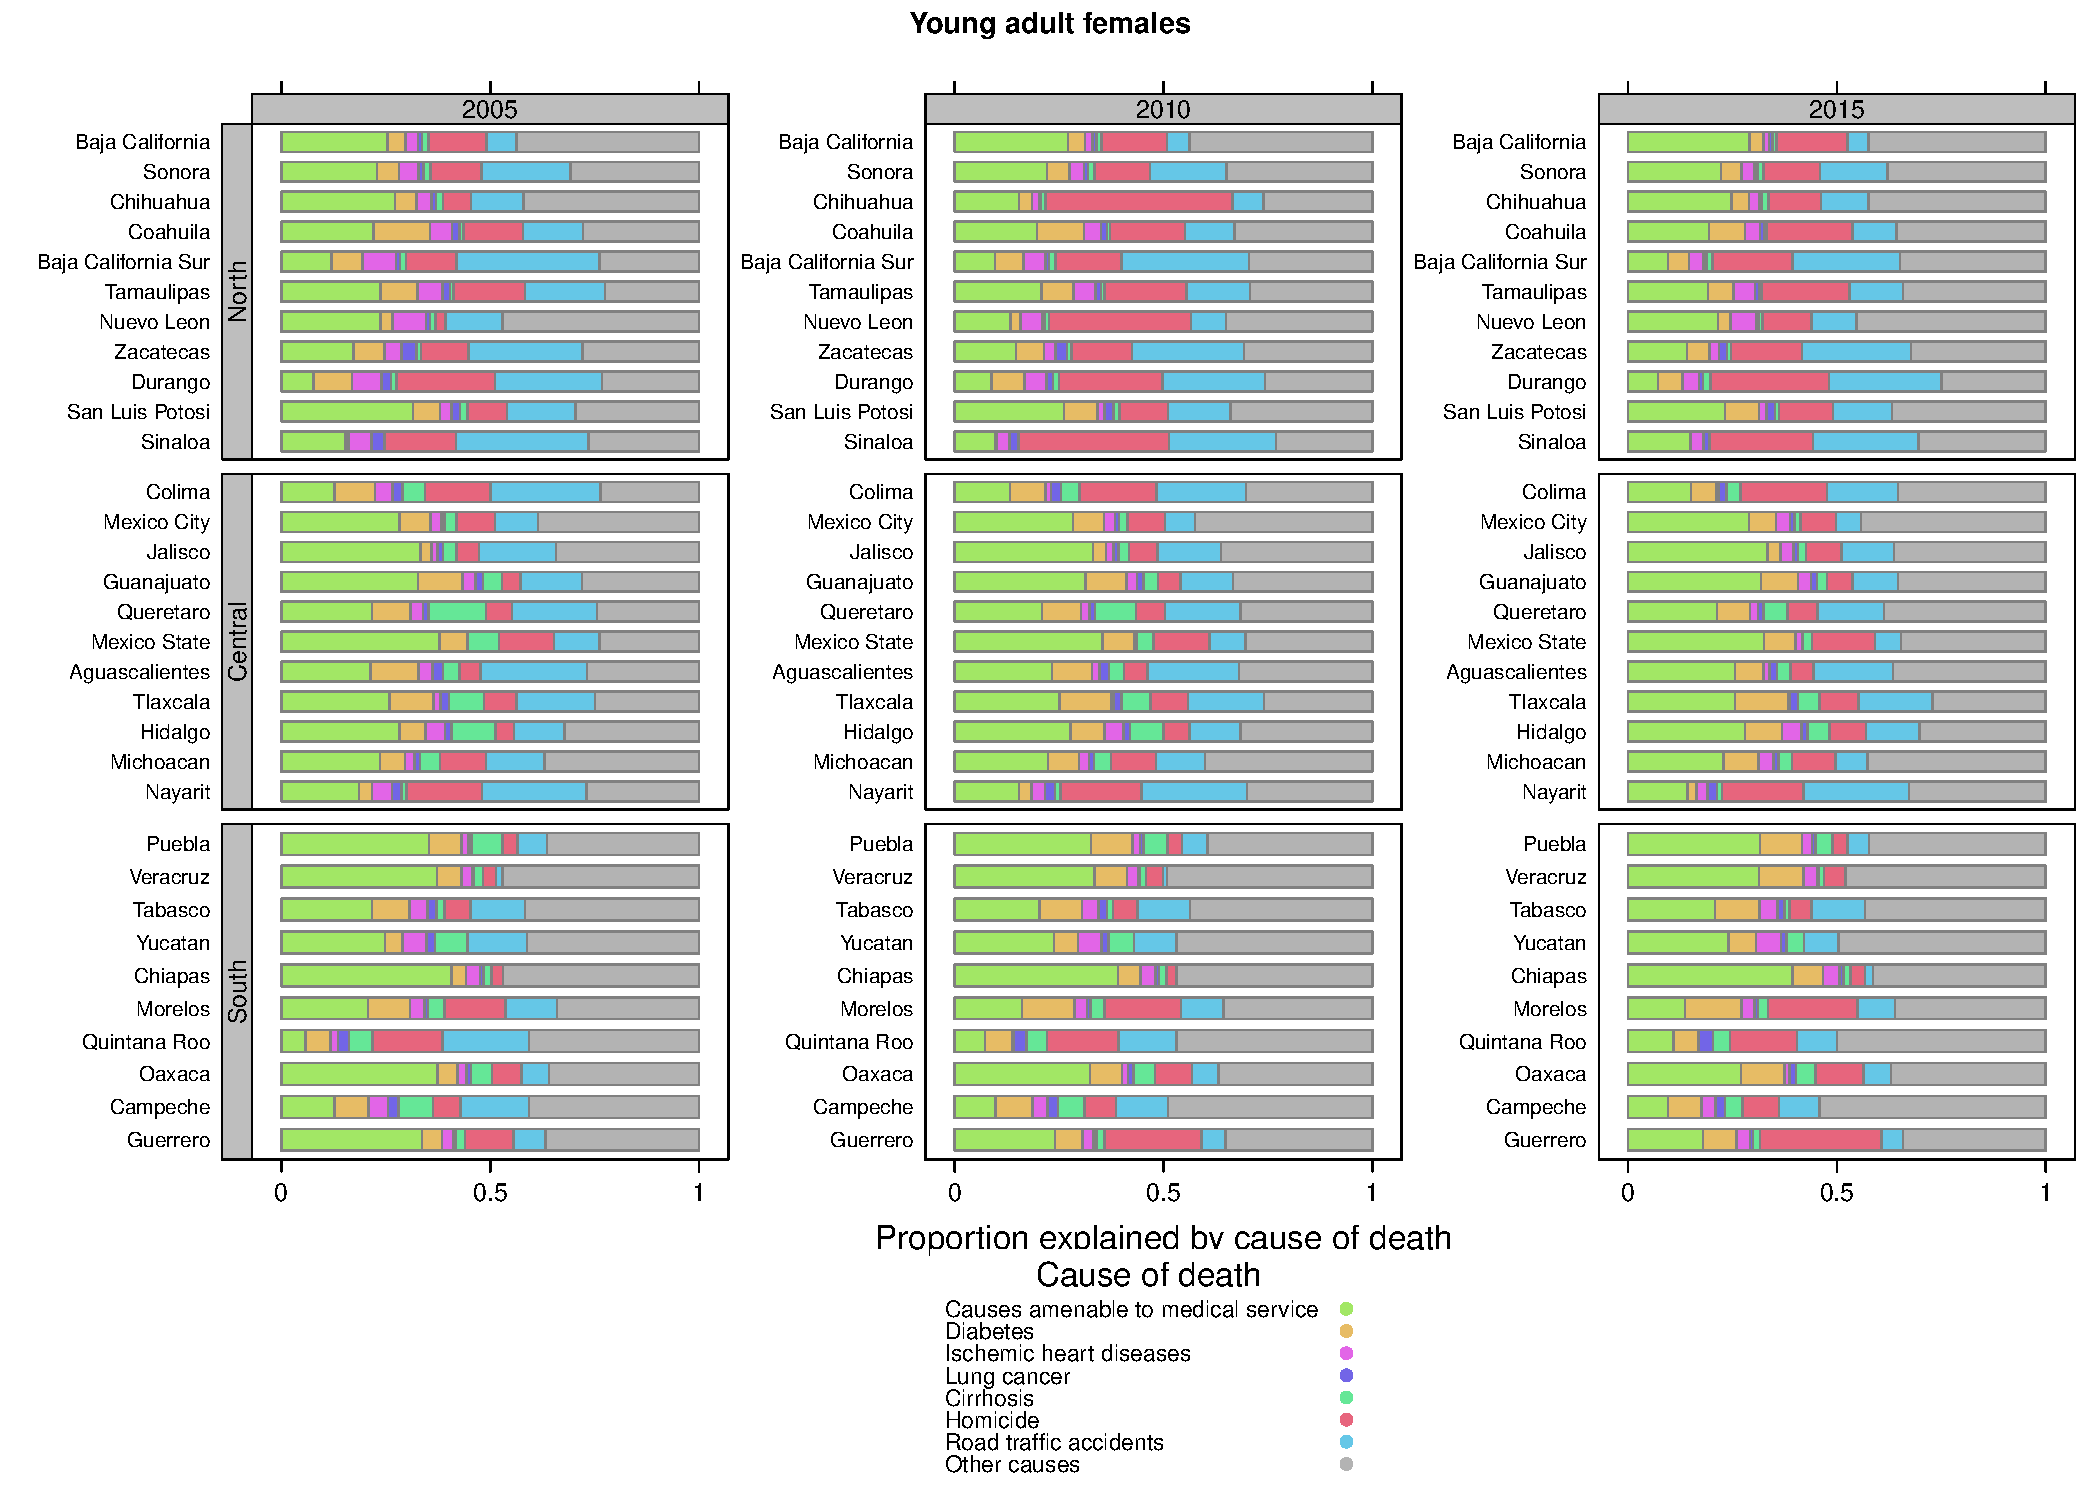
\includegraphics[scale=.45]{Figure_prop_yaf.pdf}
\end{center}
\end{figure}


\begin{figure}
\centering
\caption{Proportion by cause of death from benchmark mortality for young adult males (ages 15-49). Source: own elaborations.}
\begin{center}
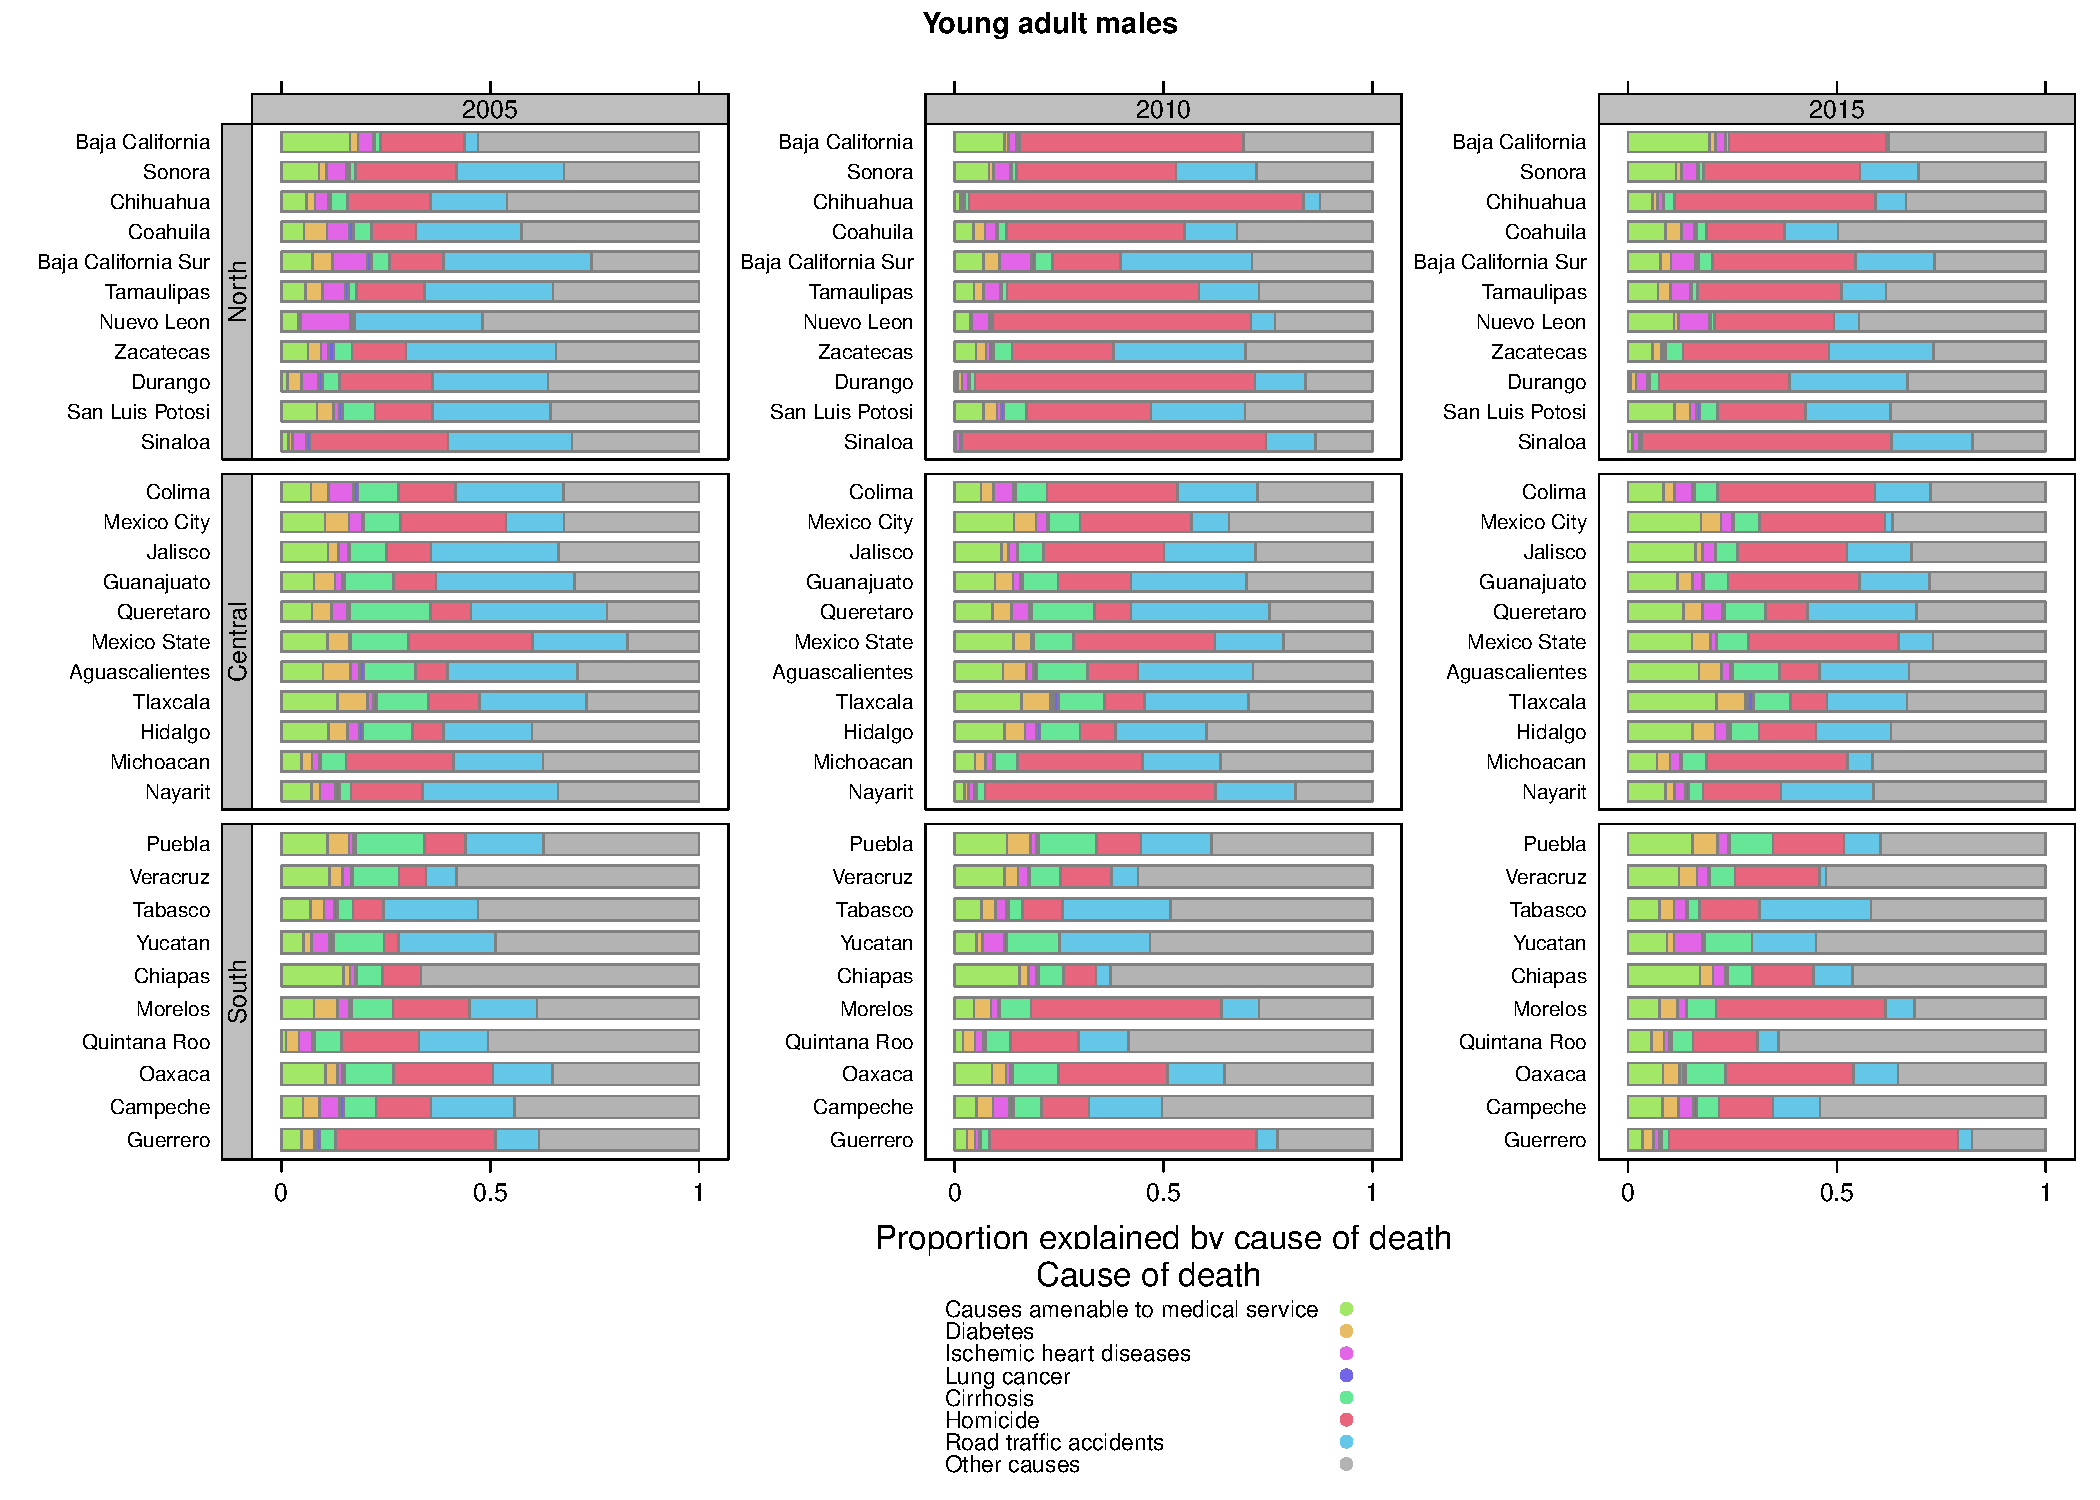
\includegraphics[scale=.45]{Figure_prop_yam.pdf}
\end{center}
\end{figure}


\begin{figure}
\centering
\caption{Proportion by cause of death from benchmark mortality for older male adults (ages 50-84). Source: own elaborations.}
\begin{center}
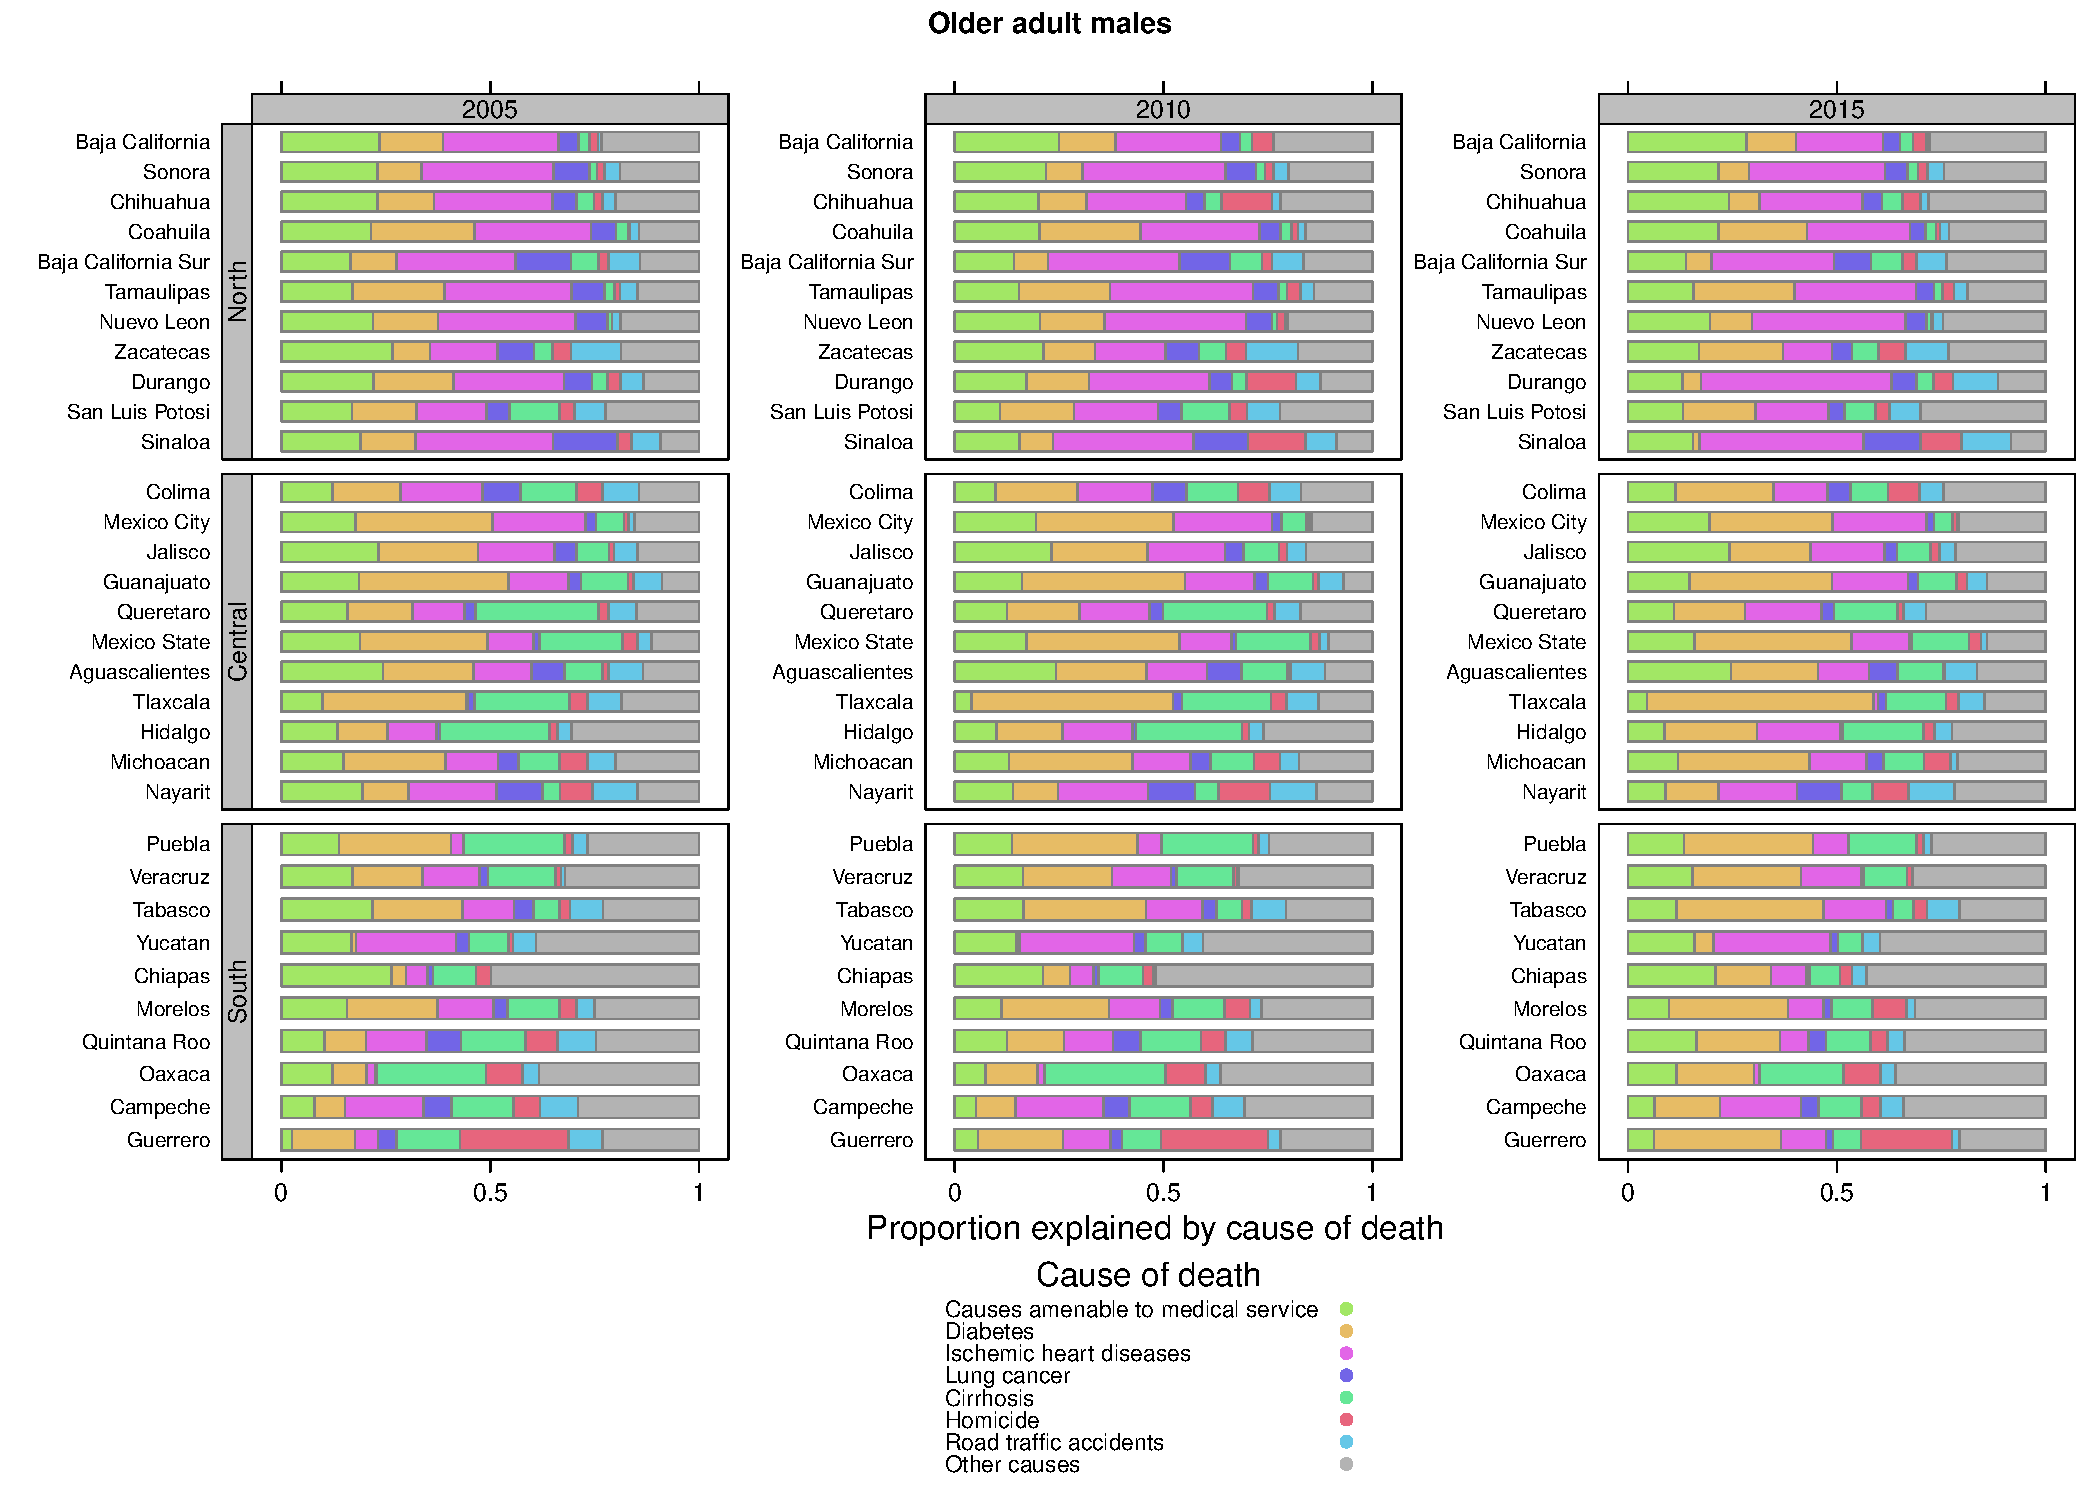
\includegraphics[scale=.45]{Figure_prop_oam.pdf}
\end{center}
\end{figure}


\begin{figure}
\centering
\caption{Proportion by cause of death from benchmark mortality for older female adults (ages 50-84). Source: own elaborations.}
\begin{center}
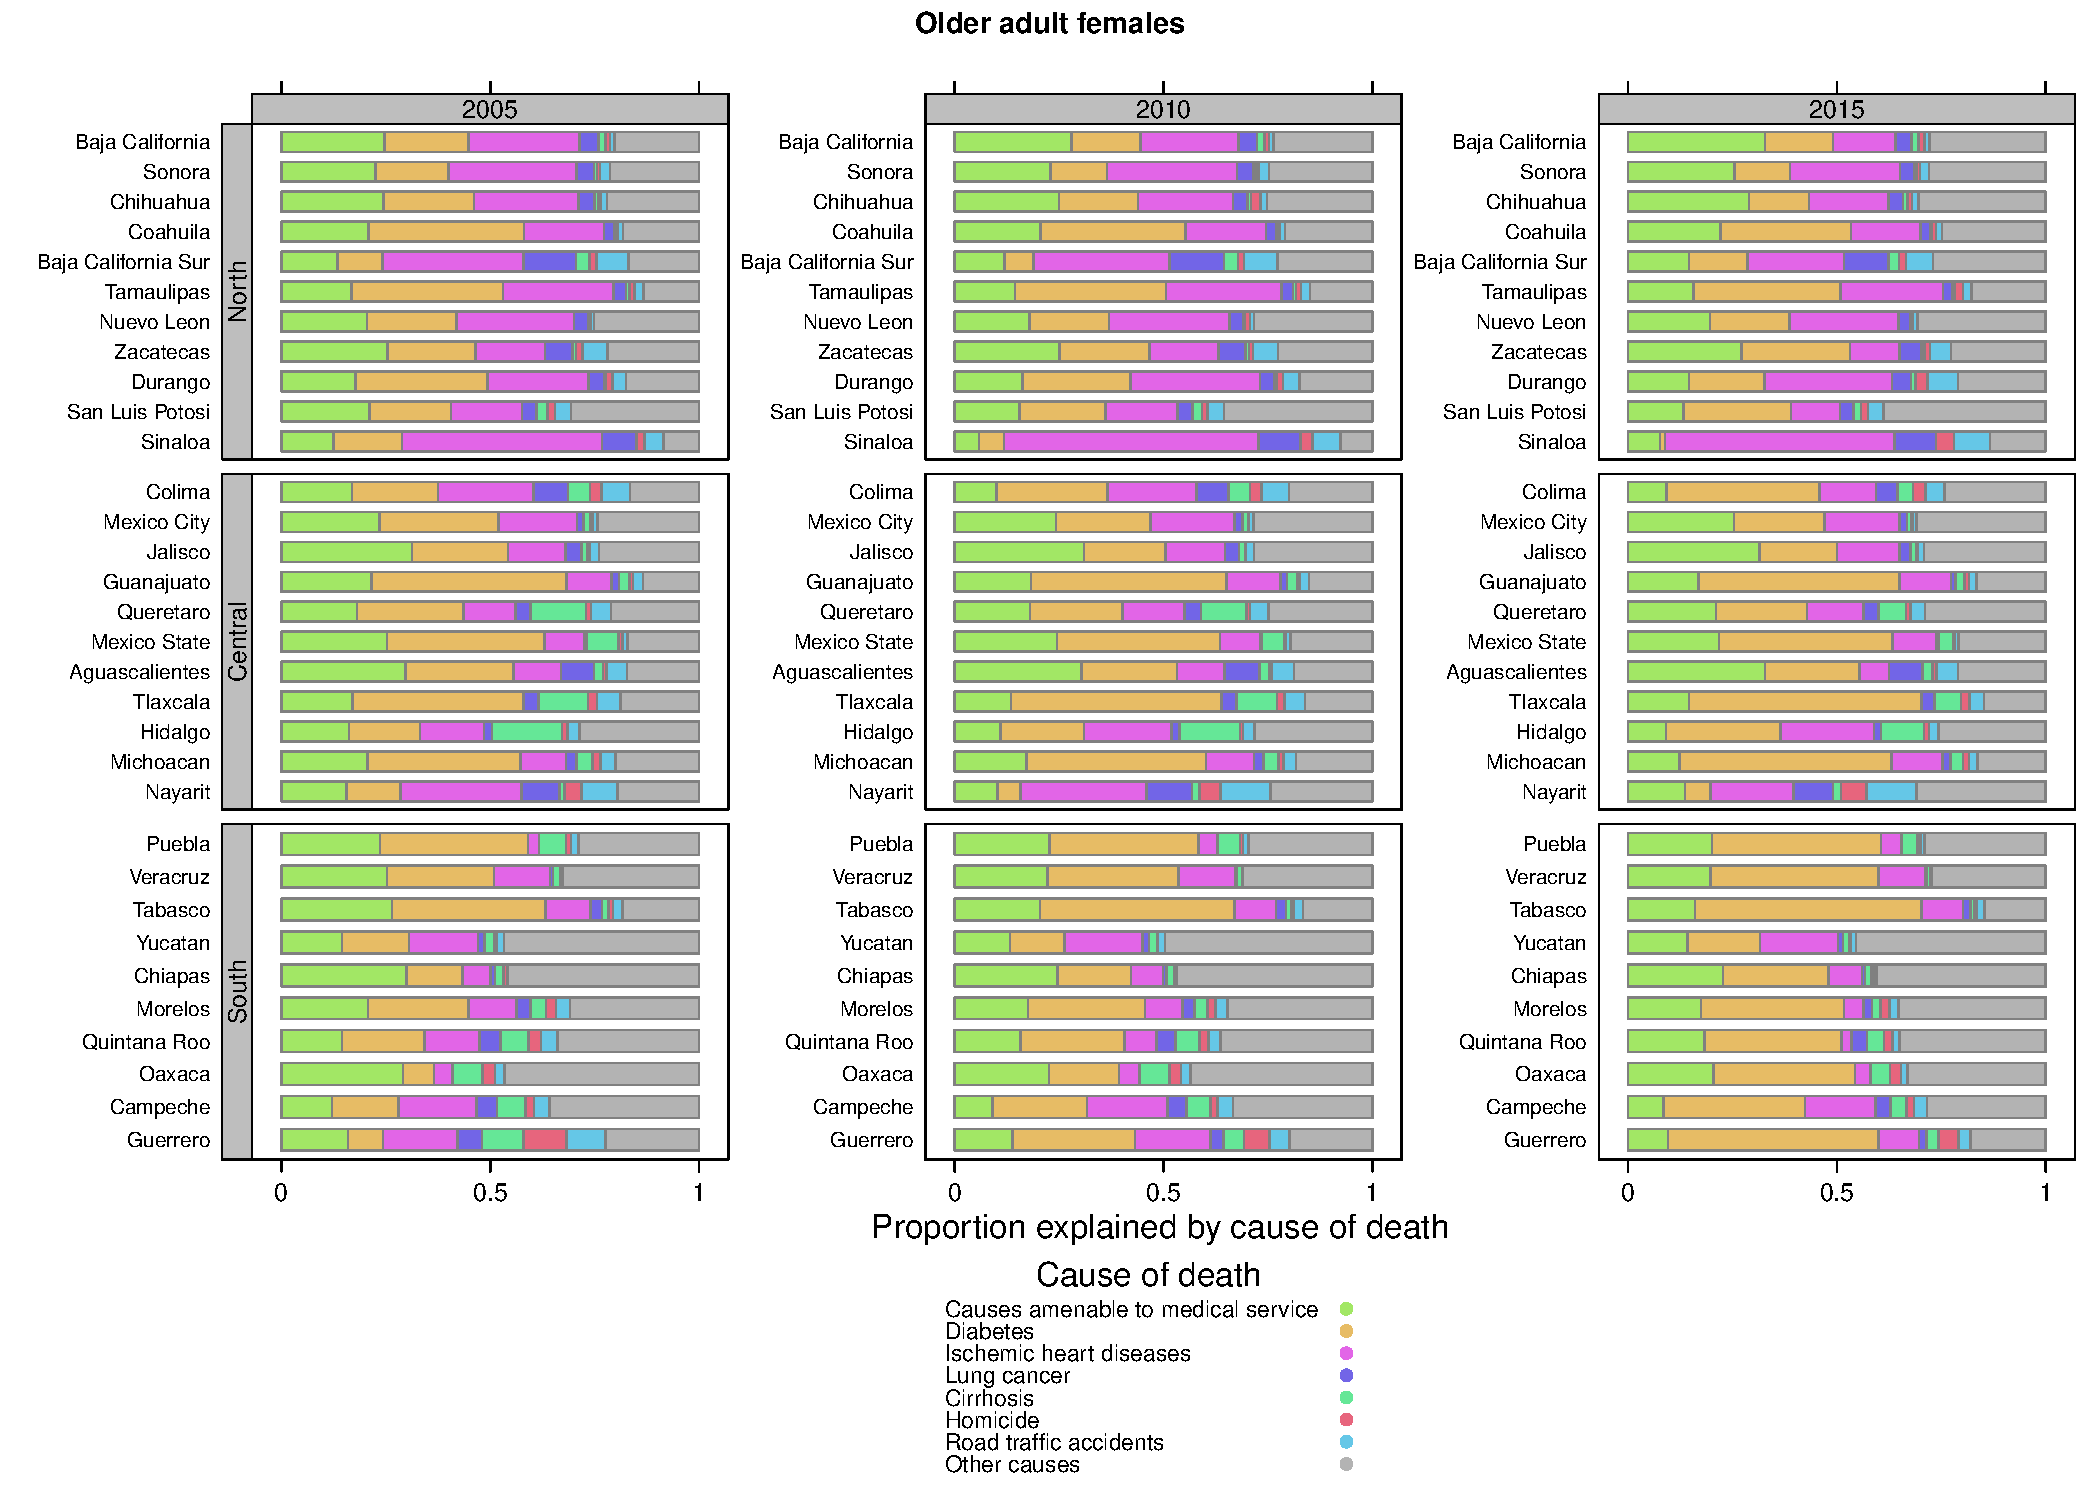
\includegraphics[scale=.45]{Figure_prop_oaf.pdf}
\end{center}
\end{figure}



\bibliography{AburtoRiffe_Bib}







\end{document}
